\documentclass[12pt]{article}
\usepackage[margin=1in]{geometry} % Create 1 inch margins
\usepackage{natbib} % Citation package 
\usepackage{indentfirst} % Indent the first paragraph of the 1st paragraph of each new section. 
\usepackage{setspace} % Package to set my line spacing
\usepackage[bottom]{footmisc}
\doublespacing % declare double space
\interfootnotelinepenalty=999999999
\usepackage{sectsty}
\sectionfont{\normalfont\fontfamily{ptm}\fontsize{12}{12}\bfseries}
\subsectionfont{\normalfont\fontfamily{ptm}\fontsize{12}{12}\itshape}
\usepackage{times} % Text font as TNR
\usepackage{graphicx} % Include images 
%\usepackage[none]{hyphenat} % Stops breaking up words at the right side of the page. 
\usepackage{comment} % Pakeage to let me comment out large secitons at a time.
\usepackage{xurl} % Fix urls on the page
\usepackage{array}
\usepackage{caption}
\usepackage{subcaption}
%\usepackage{hyperref} % Hyperlink to figures and bibliography
\usepackage{fancyhdr} % All of this is to put the page number at the bottom right
\usepackage{titling}
\pagestyle{fancy}
\fancyhead{}
\fancyfoot{}
\fancyfoot[R]{\thepage}
\renewcommand{\headrulewidth}{0pt} % This says to not put the line at the top of the apge that makes it "fancy".
\setlength{\parindent}{1cm}
\renewcommand{\thesection}{\Roman{section}}
\renewcommand{\thesubsection}{\thesection.\Roman{subsection}}
\usepackage{soul} % Fix wrapping of underlined text
\usepackage[font=small]{caption} %Change the size of the "Figre XX" caption part. 
\usepackage{xcolor}
\usepackage{import}
\usepackage{tikz,pgfplots}
\usepackage{tkz-graph}
\usetikzlibrary{arrows.meta}
\usetikzlibrary{positioning}

%%% Paper Info %%%%
\title{UN-Interested Suppliers \\
\large Effects of Peacekeeping Mandates on Contributions}
\author{Trey Wood \\
University of Kentucky}
\date{\today}


\newcommand{\fix}[1]{\section{FIX}\LARGE\color{red}#1}
\newcommand{\Dan}[1]{\par\color{red}\underline{Note for Dan:} \color{black}#1}
\providecommand{\keywords}[1]{\center\textbf{\textbf{Key words:}} #1}

\begin{document}

\begin{titlingpage}
\maketitle
\begin{abstract}
\begin{singlespace}
Why do troop contributing countries differ in their contribution levels across missions? States that make contributions have the flexibility to select which missions their troops will join while retaining the authority to recall their troops. The literature notes that contributions are influenced by international and domestic factors, but it fails to explain how mission specific factors affect contributions. I argue that when mission mandates contain tasks that signal the potential for peacekeeper injury or death, states send smaller contributions to the risky mission, which is further exacerbated by increasingly dangerous conflict environments. Using the Tasks Assigned to Missions in their Mandates (TAMM) dataset, I find that states provide smaller contributions when mandates contain a large proportion of risky tasks, which becomes increasingly small as the conflict environment becomes more dangerous. This study demonstrates that states consider both mission mandates and conflict environments when contributing to United Nations peacekeeping operations.
\end{singlespace}
\end{abstract}
\begin{center}
\textbf{Keywords:} United Nations, Peacekeeping, Mandates, Troop Contributions \\
\textbf{Words Used:} 10,348 words
\end{center}
\end{titlingpage}

\newpage

\begin{comment}

THANK PEOPLE
Dan for comments
Clayton for comments
The Great Smokey Mountains Workshop for comments
Austin Doctor for comments
Jared Oestman for comments
ISA-MW for comments

\end{comment}

In 2005, the Government of Sudan and the Sudan People's Liberation Movement/Army (SPLM/A) signed the Comprehensive Peace Agreement with plans for a south Sudanese referendum. In 2011, the referendum demonstrated that many individuals in southern Sudan supported self-determination leading to the creation of South Sudan. In response, the United Nations Security Council mandated the United Nations Mission in the Republic of South Sudan (UNMISS) to develop government institutions, promote socio-economic development, and protect civilians. Instead of focusing on external issues such as the new state's relationship with Sudan, UNMISS focused on internal issues in South Sudan \citep{PKO_UNMISS}. The Comprehensive Peace Agreement formally ended the Sudanese civil war, but it failed to finalize the division of disputed territories. Specifically, contestation erupted over the Abyei territory between Sudan and South Sudan that obstructed peace agreement implementation creating renewed conflict in 2008, which displaced over 100,000 civilians in Abyei in 2011. Later in 2011, the United Nations deployed the United Nations Interim Security Force for Abyei (UNISFA) to promote the demilitarization of the region, develop security forces, and repatriate refugees \citep{PKO_UNISFA}. 
% 189 words

%\footnotetext[0]{I want to thank Clayton Thyne and Daniel Morey for their thoughtful comments on numerous drafts of this project. I also thank the attendees of the Great Smoky Mountains Political Science Research Workshop, Austin Doctor, Jared Oestman, my classmates in PS 738, and the University of Kentucky Political Science Department Colloquium attendees for their comments on later versions of this project.}
% 61 words

Both United Nations peacekeeping missions were rooted in the same conflict and peace agreement concerning Sudan, but their average contributions were drastically different. Using contribution counts provided by \cite{perry2013}, in 2011, UNMISS averaged 29 troops per contributor month while UNISFA averaged 13 troops per contributor month. In substantive terms, Egypt in 2011 maintained an average of 604 troops in UNMISS and 7 troops in UNISFA. Furthermore, India in 2011 deployed an average continent of about 2250 troops in UNMISS in contrast to an average of 8 troops in UNISFA. In summary, UNISFA took place at the same time and stemmed from the same conflict as UNMISS, but UNISFA maintained about half the average contributions and had a noticeable difference in contributor deployments. The disparity in mission contributions motivates the research question of this study: \textit{Why do troop contributing countries differ in their contribution levels across missions?} 
% 149 words

I argue that contribution levels are a function of mission mandate tasks and the conflict environment associated with each mission. UNMISS was tasked to monitor and enforce the peace agreement, but it also had less risky tasks such as election assistance, government capacity development, and the promotion of a free press. In contrast, UNISFA had a riskier mandate with tasks that included buffer zone monitoring, peace agreement enforcement, and human rights protection \citep{lloyd2021}. The risky tasks and dangerous conflict environment of UNISFA deterred states from contributing to the hazardous peacekeeping operation while UNMISS' inclusion of relatively less risky tasks did not deter troop contributions. When mandates are less risky and the conflict environment is peaceful, states will contribute troops to receive domestic and international benefits. However, mandates that are increasingly risky and are implemented in dangerous conflict environments increase the potential costs that outweigh the benefits of contribution leading to reduced troop contributions. Leveraging a dataset with peacekeeper troop contribution counts, mandate tasks, and a measure of conflict danger, I find that contributing states avoid sending troops to missions with risky mandates and dangerous conflict environments. 
% 187 words

This study provides implications for the academic and policy communities. For the academic community, current research demonstrates the deterrent effect of missions in terms of civilian and battle deaths \citep{hultman2013united,hultman2014beyond} and a mission's ability to create lasting peace \citep{blair2021}. However, this study finds that risky missions in dire need of resources deter the contributions necessary to limit the effects of conflict. For policymakers, peacekeeping operations have become the preferred mode of international intervention and peace development \citep{UN_SC}, but state contribution reductions as a result of mission specific factors limit the United Nations' conflict management potential due a deficit of resources required to credibly threaten force for peace. This study raises the issue that the most desperate peacekeeping missions are detrimentally under-supplied leading to ineffective missions. 
% 133 words

\section*{The Process of Troop Contributions}

Though peacekeeping operations and their mandates are formed on a ``case-by-case'' basis, the United Nations follows a similar bureaucratic process regarding mission formation \citep{UN_SC}. This suggests that missions share similar problems in various stages, specifically collective action problems when gathering troop contributions. Noting this problem, scholars have discovered domestic and international factors that states leverage to promote contributions. However, the literature has not evaluated how mandate risk affects contributions, defined below. 
% 74 words

\subsection*{Mission Formation}

The United Nations Security Council has the primary responsibility to authorize peacekeeping deployments and their mandates. After observing inter- or intrastate war and deciding to intervene, the United Nations Security Council must pass a resolution to form a mission with its associated mandate \citep{UN_SC}. The mandate, legally based in Chapters VI and VII of the United Nations Charter, iterates tasks tailored to each case to support peace and security. These tasks include mission objectives such as conflict spillover prevention or peace agreement enforcement. In contrast to violence limiting tasks, other tasks such as disarmament, demobilization, and reintegration of ex-combatants and human rights protections fall under the umbrella of peace-building activities. In extreme cases, the Security Council can leverage Chapter VII of the Charter to authorize peace-enforcement for effective mandate implementation without intervention consent from the warring parties \citep{mandate.online}, which has become increasingly common since 1999 \citep{howard2018use}. In short, missions are mandated with tasks to support the goal of peace promotion and host state restabilization. 
% 171 words

%\footnotetext[1]{\doublespacing \fontsize{12}{12}\selectfont If the Security Council does not send a mission due to a permanent five member veto, the General Assembly can authorize a mission, but this power was only invoked in 1956 when the General Assembly established the First United Nations Emergency Force (UNEF I) \citep{UN_GA}.}
% 48 words

After creating the mandate, the United Nations gathers the necessary resources for deployment. United Nations member-states have two roles in burden sharing for United Nations peacekeeping operations: financial and troop contributions. Each fiscal year, member-states are allocated a portion of the United Nations budget to pay based on the member-state's relative economic wealth and permanent membership status on the Security Council, among other criteria. These financial contributions are split between various United Nations budgets, including the peacekeeping budget \citep{coleman2020}. Due to the compulsory nature of this aspect of burden sharing, missions are more likely to have the necessary financial resources to build and support peacekeeping operations.\footnotemark[1]
% 108 words

\footnotetext[1]{\doublespacing \fontsize{12}{12}\selectfont Many member-states make late payments even though they are legally obligated to contribute. In the event of budget shortfalls, the United Nations will operate with a tight budget and utilize cash and other reserves to fund missions until payments are made \citep{generalassembly_2021}.}
% 44 words

In contrast to financial contributions, the voluntary nature of troop contributions often lead to under-supplied missions. Peacekeeping operations suffer from collective action problems as the goal of conflict resolution and peace is non-rivalrous and non-excludable \citep{boncheck1997}. The United Nations does not keep a standing army for conflict intervention, creating a reliance on member-states contributions. After a mission is mandated by the Security Council, the Department of Peacekeeping Operations negotiates with member-states to gather troops and resources for the mission \citep{allen2014}, but member-states are not required to contribute troops. Knowing this, the Department of Peacekeeping Operations offers a monthly reimbursement to the contributing country in exchange for their troops \citep{united_nations}. However, the reimbursement cannot entice all member-states to contribute due to the cost of a soldier \citep{bove2011}, an inability to match inflation, or reimbursement backlogs from peacekeeping budget shortfalls \citep{coleman2018}. The voluntary nature of peacekeeping presents member-states the opportunity to free-ride off the contributions of other member-states. 
% 168 words

Should a member-state decide to contribute to the mission, states will decide not only how many peacekeepers to send, but also which missions they want to supply with the understanding that their troops can be recalled at any time \citep{united_nations}. The contributed troops do not give their loyalty to the force commander, but rather acquiesce to the commander's operational control. This means that the troops may be directed by the force commander while on mission, but the troops continuously remain under command of their native government, even to the point of withdrawal from the mission \citep{leck2009}. This implies that in the context of contributions, troop contributing countries have flexibility. When a mission opportunity arises, member-states have the flexibility to choose whether to contribute troops to a mission, to which missions their troops will be deployed, and whether or not to withdraw or reduce their contributions.
% 148 words

\subsection*{Drivers of Contributions}

Even though member-states are not required to contribute to a mission, the benefits associated with contributions can entice troop burden-sharing. The benefits of monthly troop reimbursements, which is about \$1,410 per troop per month as of July 2017 \citep{UN_deploy}, and coup-proofing are major drivers of troop contributions, often drawing poor, autocratic states to participate \citep{gaibulloev2015,kathman2017,duursma2019,levin2021test}. Many member-states engage in ``peacekeeping for profit"\footnotemark[2] as reimbursements are used to stabilize the state by supplying private goods to potentially troublesome military officers \citep{gaibulloev2015, kathman2017,lundgren2018}. If reimbursements do not quell the disgruntled officers, states can deploy them to a mission to disrupt the coup network \citep{hesse2015,kathman2017,levin2021test}. After the 1990s, a reduced need for coup-proofing \citep{levin2021test} and the threat of conflict violence deterred democratic troop contributions leading to the ``mercenarization" of autocratic militaries to fill this contribution gap \citep{bove2011,duursma2019}. 
% 178 words

\footnotetext[2]{\doublespacing \fontsize{12}{12}\selectfont \cite{coleman2018} suggest the ``peacekeeping for profit" narrative holds only when contributors acquire stocks of old equipment and are paid a modest deployment allowance.}
% 26 words

In addition to domestic effects, states are also motivated to contribute by international factors. By leveraging information gathered from international institution linkages \citep{joshi2020}, pivotal states\footnotemark[3] can entice other member-states to contribute by supplementing troop reimbursements with foreign aid \citep{boutton2020,oestman2021price}, reputation improvements and recognition by the international community \citep{neack1995peace,hesse2015,meiske2017peacekeeping,levin2020}, or by leveraging their foreign policy similarity \citep{ward2016}. Upon deployment, contributed troops receive arms and artillery instruction to train or maintain force readiness \citep{kathman2017}. Within the United Nations, mission participation makes a state more likely to be selected to contribute a Force Commander or a Special Representative of the Secretary-General \citep{oksamytna2021} and decreases the risk of replacement given poor leadership performance \citep{lundgren2021}. Even with these enticements, states have incentives to free-ride when missions have multiple contributors \citep{bove2011}, creating mission shortfalls that hinder mandate implementation \citep{passmore2018}. 
% 163 words. CHECK LATER

\footnotetext[3]{\doublespacing \fontsize{12}{12}\selectfont Pivotal states are unwilling to deploy their troops due to contribution costs but have the power to secure foreign aid for contributing states \citep{boutton2020}.}
% 27 words

Scholars have developed a thriving literature on peacekeeping contributions, but it has paid little attention to mission specific factors. Contributing countries participate on a case-by-case basis \citep{leck2009,allen2014} suggesting that countries consider the risk associated with specific missions \citep{bullion1997india}. While the literature has considered mission specific factors, such as peacekeeper fatalities \citep{bove2011,levin2021}, it lacks an investigation of mission mandates. The risk to peacekeepers generated by mission mandates deter states from contributing to avoid the costs of fatalities thereby limiting a mission's ability to reduce civilian killings, sexual violence, and battle deaths \citep{hultman2013united,kirschner2019does,hultman2014beyond}. As a result, missions that are in most dire need of peacekeepers will be the most under-supplied and unable to create peace. I address this gap in the literature by explaining how mandate risk and conflict conditions lead to reduced contributions after a brief comment on peacekeeping mandates and risk. 
% 169 words

\subsection*{Defining Mandate Risk} 

Peacekeeping mandate tasks subject peacekeepers to increased risk in terms of their physical security. Peacekeepers on mission confront forms of risk such as the risk of war recurrence \citep{fortna2008}, terrorist attacks \citep{hansen2020}, and post-mission mental conditions including post-traumatic stress disorder and alcohol dependence \citep{forbes2016}. However, the risk of death or injury is the most important form in the context of this investigation. Conor Foley, a former evaluator in the Department of Peacekeeping Operations, finds that the United Nations' emphasis on protecting civilians through the authorization of offensive operations and robust mandates\footnotemark[4] coincide with peacekeepers moving to conflict locations such as villages and buffer zones where risk is much higher \citep{martin_2018}. Troop-contributing countries realize the risk associated with specific mandate tasks and mission locations leading to the concern for their troops \citep{karlsrud2015,henke2019}. With this in mind, I define ``risk" as the likelihood of a peacekeeper being killed or injured while implementing the mission mandate. Table 1 presents the division of peacekeeping mandate tasks that are considered ``risky'' and ``less risky.''
% 180 words

\footnotetext[4]{\doublespacing \fontsize{12}{12}\selectfont The United Nations characterizes a robust mandate as one that allows ``the use of force by a United Nations peacekeeping operation at the tactical level, with authorization of the Security Council, to defend its mandate against spoilers whose activities pose a threat to civilians or risk undermining the peace process," \citep{hiller_2020}.}
% 52 words

When classifying tasks as ``risky'' or ``less risky,'' I identify tasks where peacekeepers are likely to be targets of conflict, likely to use force in protection of the mandate, or engage in naturally risky tasks as these situations are most likely to lead to peacekeeper death or injury. Peacekeepers who monitor buffer zones or patrol local villages are likely to be targets of warring parties should the parties engage in some level of conflict \citep{fjelde2019,townsen2014}. In addition, peacekeepers tasked to monitor state borders and natural resource deposits are likely to be targeted due to rebel group border hoping and conflict over financial opportunity, respectively \citep{beardsley2011,townsen2014}. Some mandate tasks demand that peacekeepers protect civilians, human rights, and United Nations and humanitarian mission personnel through the use of force \citep{hultman2013united}. Last, some tasks such as warring party demobilization and demining assistance are situations that are inherently dangerous due to occupational hazards associated with the task \citep{DDR,demining}. A detailed explanation of the division of these tasks can be found in Appendix E. In summary, risky tasks are those that make peacekeepers potential targets of conflict, demand the use of force, or are naturally dangerous. 
% 211 words

%\begin{center}
\begin{table}[t]\centering
\fontsize{7.5}{7.5}\selectfont
\def\sym#1{\ifmmode^{#1}\else\(^{#1}\)\fi}
\caption{Table of Task Risk}
\label{Table 1}
\begin{tabular}{c*{2}{c}}
\hline\hline
                    \multicolumn{1}{c}{Risky}         &\multicolumn{1}{c}{Less Risky}      \\
\hline \\
Monitor Peace Agreements                                & Promote Good Offices (Subtask of Monitor Peace Agreements) \\
Subtasks: Buffer Monitor and Liaise War Parties         &  \\
[0.5em]
Monitor Human Rights                                    &   Monitor the Weapons Trade, Monitor Weapons Embargo, \\ 
Subtask: Monitor the Refugee Situation                  & Inspect Cargo (Subtasks of Monitor Borders) \\ 
[0.5em]
Protect Human Rights                                    & Monitor Use of Natural Resources \\
Subtasks: Protect Children, Protect Women,              &  \\
Protect Civilians                                       & \\
[0.5em]
Protect UN Personnel (Ensure Security)                  & Monitor Elections \\
[0.5em]
Assist in Demining                                     & Provide Security During the Electoral Period\\     
[0.5em]
Monitor Borders                                         & Assist with Election Implementation \\
                                                        & (Technical or Logistical Assistance) \\
[0.5em]
Chapter VII Authorization                               & Build Government Capacity \\
                                                        & Subtask: Implement Government Policies \\
[0.5em]
Assist with Security Sector Reform                      & Preserve Cultural and Historical Sites \\ 
Subtasks: Assist Police Reform, Monitor the Police,     &   \\
Conduct Joint Patrols with Police                        &   \\ 
[0.5em]
Monitor Disarmament, Demobilization,                    & Assist in the Implementation of Quick Impact Projects (QIP) \\
 and Reintegration                                      & \\
[0.5em]
Help Implement Disarmament, Demobilization,             & Assist with Justice Sector Reform \\ 
and Reintegration                                       & \\
[0.5em]
                                                        & Promote National Reconciliation \\
                                                        & Subtask: Pursue Justice for War Criminals \\
[0.5em]
                                                        & Disseminate Info About the Mission to the Public \\
[0.5em]
                                                        & Promote Freedom of the Press \\                                                                            
\hline\hline
\multicolumn{1}{l}{\footnotesize Table adapted from tasks coded in Lloyd (2021).}\\
\end{tabular}
\end{table}


%\end{center}
% 175 words

\section*{Mandate Tasks and Contributions}

\indent Compared to the number of wars observed in the international system, peacekeeping is relatively rare and deploys to the most difficult conflicts. \cite{fortna2008} finds that only 38\% of post-Cold War civil wars experienced a United Nations deployment.\footnotemark[5] The United Nations Security Council prioritizes deployments to ``hard cases," meaning civil conflicts that lack a decisive victory that experienced high battle deaths counts and previous mediation attempts \citep{gilligan2003, fortna2004, mullenbach2005}. These types of conflicts suffer from information asymmetries and commitment problems that prevent conflict termination or hinder long-term post-conflict peace \citep{walter2009}.   
% 96 words

\footnotetext[5]{\doublespacing \fontsize{12}{12}\selectfont Mission types range from observer missions without the authorization to use force, Chapter VI missions with an emphasis on peace building, and Chapter VII missions that intend to force peace during conflict \citep{PKO_Ox}.} 
% 34 words

Once peacekeepers arrive in the most difficult host states, troops deploy to dangerous locations within the host state. When on mission, peacekeepers deploy to hotspots of conflict that include host state borders and surface-based natural resource deposits as these locations are home to rebel transnational movements and conflict over loot, respectively. Peacekeepers also move to zones of rampant one-sided violence \citep{fjelde2019} and arenas of government and rebel troop head-to-head combat \citep{phayal2020} to protect civilians from physical harm. If peacekeepers are not already near these locations, they are stationed near transportation networks for rapid response \citep{townsen2014}. The trend of missions going to dangerous host states and conflict zones demonstrates that United Nations military leadership is risk-acceptant in conflict. 
% 126 words

\subsection*{States Sometimes Rise to the Occasion}

State participation in international institutions, such as through peacekeeping troop contributions, shows the perceived benefits of contribution are greater than its perceived costs. When international institution participation demands little to no behavior change or has few costs associated with participation, states participate in international institutions to receive cooperation benefits \citep{downs1996}. When the provision of benefits is not credible or too small to outweigh the costs in the bargain enforcement stage, then states will not expend resources in the bargaining phase \citep{fearon1998}. In the pre-contribution stage, the United Nations bargains with potential contributor countries to create a memorandum of understanding. This agreement establishes expectations regarding troop contributions and mission responsibilities as well as the expected reimbursements for the member-state \citep{Deploy} in the enforcement stage. Should a member-state find the benefits outweighed by the costs, the state will not bargain with the United Nations over contributions. 
% 150 words

When member-states decide to send troops to a mission, states receive both international and domestic benefits associated with contribution. Domestically, states receive the benefits of troop training, coup-proofing, and monthly reimbursements \citep{kathman2017,lundgren2018}. Internationally, states receive the benefits of foreign aid considerations, international prestige, and peacekeeping leadership opportunities \citep{boutton2020,levin2020,lundgren2021,oksamytna2021}. When potential costs are minimal, states prefer to contribute and provide larger contributions to peacekeeping operations to receive domestic and international benefits \citep{bobrow1997maintaining}. However, as the costs, or prospective costs, of contribution increase, states will decrease or even withdraw their respective troop contributions. 
% 112 words

\subsection*{Risk-Averse Contributors}

When deciding to contribute troops, states weight the prospective costs in light of the benefits of participation. While battle death tolls in civil conflict have decreased overtime \citep{nils2016}, the increase in peacekeeper deaths since 2000 \citep{henke2019} has contributed to the risk-aversion of states that fear losing troops to conflict violence.\footnotemark[6] Deploying troops into a conflict environment exposes troops to the risk of being injured or killed as a product of the conflict. States place a high value on the life of a soldier due to state investments in training and the costs associated with troop replacement. As a result, states are risk-averse when sending troops into conflict \citep{bove2011} as losing troops in one conflict restricts the contributor's force supply \citep{von2008}. When peacekeepers are killed on mission, states incur not only human and material costs \citep{oestman2021price}, but also domestic reputational costs as states must justify the loss of life to their audience \citep{page2016}.\footnotemark[7] Peacekeeper deaths also embolden rebel groups to continue to kill peacekeepers as troop deaths are perceived as a sign of weakness \citep{levin2021}. States as mediators avoid cases that are difficult or are expected to be unsuccessful \citep{iwanami2014}, such as when the conflict situation becomes increasingly violent. As a result, states will be incentivized to withdraw or reduce their contributions as the presence of risk increases to avoid costs.
% 233 words

\footnotetext[6]{\doublespacing \fontsize{12}{12}\selectfont Former force commander Lieutenant General (Retired) Carlos Alberto dos Santos Cruz admits that peacekeepers are constantly threatened with hostile acts from armed groups, terrorists, organized crime, and other threats causing troop contributing states to reduce their contributions as ``some T/PCCs remain risk-averse and unwilling to use force, leaving attacks unpunished and undeterred," \citep[11]{Improve_Security}.}
% 59 words

\footnotetext[7]{\doublespacing \fontsize{12}{12}\selectfont In 2016, two Chinese peacekeepers were killed in a refugee camp. China's Defense Ministry ``strongly condemned" this use of violence, but Chinese online users asked, ``What use is condemnation? ... Fight those who have injured us, don't just condemn!" \citep{page2016}.}
% 47 words

In 2014, the General Assembly authorized the Secretary-General to reward risk premiums to troop units that ``are operating without restrictions and caveats imposed by troop- and police-contributing countries and that have acquitted themselves well despite exceptional levels of risk." The premium is no greater than 10\% of the standard monthly reimbursement rate. To receive this premium, units must be free of contributor caveats, units must experience ``exceptional levels of risk," and units must perform beyond the call of duty and execute their tasks with a high level of skill and professionalism. If the unit under consideration has engaged in any form of misconduct, it cannot be rewarded with risk premiums \citep{razza_2020}. The United Nations does not publicly record risk payment rewards, but due to the extensive process of recommending units to be rewarded and the arduous review process, risk premiums seem to be rare. Furthermore, a 10\% bonus of about \$141 that is paid at the end of service is likely to be non-motivating.
% 164 words

With the risk-aversion of states in mind, mandates that imply risky peacekeeper action causes states to decrease their contribution, which is further exacerbated by the conflict environment. When the United Nations Security Council passes a resolution, the mission is charged with assorted mandate tasks\footnotemark[8] with varying prospects of risk. Mission mandates include tasks that communicate how troops are expected to engage with the warring parties and the domestic population while on mission \citep{di2022introducing}. While each task communicates some level of risk, states observe mission mandates as an aggregation of all tasks. This aggregation signals to states the level of risk associated with implementing the given mandate and the prospects of losing troops to mandate implementation. As a result, mandates with tasks that communicate high levels of risk receive smaller contributions than those with low levels of risk. 
% 141 words

\footnotetext[8]{\doublespacing \fontsize{12}{12}\selectfont A task is a mission action that relates to some actor, institution, or process \citep{lloyd2021}.} 
% 16 words

To further explain how tasks communicate risk, I draw on the monitor buffer zone task found in Table 1. The buffer zone monitoring task requires peacekeepers to patrol to areas of high risk. Buffer zones mark territory that warring parties cannot cross to deter aggressive action, but the peacekeepers who monitor the buffer zone risk being sandwiched between combatants. While monitoring the buffer zone in Cyprus, peacekeepers experience approximately 1,000 incidents each year with issues that include name-calling, the unauthorized use of firearms \citep{Aboutthe17:online}, and patrol vehicle attacks \citep{UN_CYP_2022}. The desolate territory also attracts illegal hunting creating fear among peacekeepers that a stray bullet will reignite conflict \citep{UNFICYPw80:online}. The Israel-Syria buffer zone also experienced peacekeeper kidnappings in 2013 and 2014 \citep{PKO_UNDOF} in addition to interstate skirmishes leading to United Nations condemnation regarding the use of force in the buffer zone. The task of monitoring a buffer zone signals to contributors increased levels of risk in the mandate, which is compounded by a dangerous implementation environment.
% 172 words

In contrast to risky tasks, mandate tasks such as election monitoring are comparatively low risk tasks \citep{Election}. Election monitoring requires the mission to protect elections from tampering to support the host state political process. Tasked with election monitoring in 2006, the United Nations Stabilization Mission in Haiti (MINUSTAH) delivered election materials to 9,200 polling stations to safeguard local leadership elections despite small, isolated incidents of violence \citep{UN_election}. This relatively easy task does not require troops to move to areas of conflict, especially since elections normally take place once conflict has subsided \citep{fjelde2021protecting}. This easy task matched with a safe implementation environment makes this a low-risk task for contributors looking for peacekeeping benefits.  
% 118 words

Mission mandates provide information regarding the expected actions of their troops while on mission. Knowing that contributing states base their contributions on the risk signaled by the mission mandate, states are deterred from sending troops to missions with risky mandates. High risk mandates increase the potential costs of contribution leading to reduced contribution benefits and troop contributions. This leads to the first hypothesis: 
% 63 words

\begin{center}
\begin{singlespace}
\textit{H1: As the proportion of risky tasks in the mandate \ul{increases}, the number of contributed troops will \ul{decrease}.}
% 18 words
\end{singlespace}
\end{center}

Mission mandates signal information to contributors about the risky actions expected of their peacekeepers while conflict environments communicate the difficulty associated with mandate implementation. Drawing on the argument of \cite{downs1996}, states are more likely to participate in institutions for benefits when costs are low. In the context of peacekeeping operations, the potential costs of contribution increase as mandate risk increases. Furthermore, when situations arise that demand risky mandate implementation, such as warring party clashes \citep{phayal2020}, peacekeepers will move to those locations to enforce their risky mandate. This suggests that increased conflict danger will make the implementation of a risky mandate increasingly difficult. Since peacekeeping units are smaller than the forces of the warring parties, peacekeepers must rely on comparatively unsuccessful coercive strategies \citep{sullivan2007war} against highly resolved warring parties \citep{lloyd_diss}. As a result, contributor states will send smaller contributions when mandate risk is high and the conflict environment is increasingly dangerous to avoid losing peacekeepers that attempt to implement the mission's risky mandate since states avoid intervention in difficult cases \citep{iwanami2014}. This leads to the second hypothesis:
% 185 words

\begin{center}
\begin{singlespace}
\textit{H2: As the level of conflict danger in the conflict environment \underline{increases}, the \underline{negative} effect of the proportion of risky tasks in the mandate on the number of contributed troops will \underline{strengthen}.} 
% 32 words
\end{singlespace}
\end{center}

Knowing the costs and benefits associated with contributions, states must make a difficult decision. Potential contributing states observe mission mandates that signal the potential costs of contribution as risky mandates increase the likelihood of losing troops. Increased mandate risk deters states from contributing to difficult missions. In addition to the information gleaned from mission mandates regarding troop activities that communicate risk, dangerous conflict environments signal to potential contributors that the risky mandate must be implemented in a difficult conflict environment further compound the deterring effects of risky mandates on troop contributions. 
% 91 words

\section*{Research Design}

To test the implications of the theory, I use the potential-contributor-mission-month unit of analysis to capture the change in contributions each mission-month. To begin, I count a potential contributor as any state listed in the Correlates of War (COW) State System Membership List \citep{COW_list}. Next, I capture each state's respective troop contribution for each possible mission the state did or did not contribute to in a given month. For example, the United States of America in November 1995 contributed 365 troops to United Nations Confidence Mission in Croatia (UNCRO) and sent 0 troops to the United Nations Angola Verification Mission (UNAVEM I). The United States sent troops to UNCRO, but it also had the potential to send troops to UNVAEM I in the same month.
% 129 words

To capture potential contributing states, I employ endogenous stratified sampling \citep{king2001logistic} from the conflict mediation literature \citep[Ex.][]{savun2008}. This strategy limits excess zeros by collecting all cases where states contributed to a mission in a given month as well as a random selection of states who did not contribute. I chose 15 randomly selected non-contribution cases since this is the sample average count of states the contribute to a mission. While two stage count models can explain excess zeros, these models are likely to estimate biased probabilities and standard errors due to rare event issues \citep{king2001logistic} from having more than ten times the number of non-contributors to contributors. Random selection of non-contributors alleviates rare event issues while also creating a representative sample of non-contributors for proper comparison.
% 134 words

The sample consists of all mission-months from 1990-2014. I exclude observer missions from the sample, such as the United Nation Integrated Office in Burundi (BINUB), as these missions are authorized for either zero or few troops leading to small contribution levels regardless of mandate risk. A list of the missions included in the sample can be found in Appendix B. Furthermore, I limit the sample to potential-contributor-mission-months with two-hundred or less battle deaths as these are extreme observations within the sample and exhibit high leverage on model estimates.\footnotemark[9] Removing these observations produces relatively conservative estimates. 
% 95 words

\footnotetext[9]{\doublespacing \fontsize{12}{12}\selectfont Appendix A provides estimates that include observations with large battle death counts. Many of these observations with large battle death counts come from the United Nations Organization Mission in the Democratic Republic of the Congo (MONUC), the United Nations-African Union Hybrid Operation in Darfur (UNAMID), and the United Nations Mission in the Republic of South Sudan (UNMISS). The models are robust to these influential observations, but I exclude these cases to avoid inflating statistical and substantive significance.}
% 77 words

\subsection*{Dependent Variable}

The dependent variable is the number of troops contributed in a potential-contributor-mission-month, which comes from the International Peace Institute's Peacekeeping Database \citep{perry2013}. This database provides information regarding which states contribute, the year and month of contribution, to which mission the state contributes, and how many troops the state contributes. I exclude counts of mission observers and civilian police as military troops are the actors most subject to mission risk. For example, mission observers are not the peacekeepers in charge of patrolling a buffer zone nor are the civilian police in charge of enforcing a peace agreement. Figure \ref{fig:Figure 1} provides a histogram of the dependent variable. Due to the over dispersion of the dependent variable, I employ the negative binomial estimator. 
% 123 words

\begin{figure}[t!]
\begin{subfigure}[h]{0.5\linewidth}
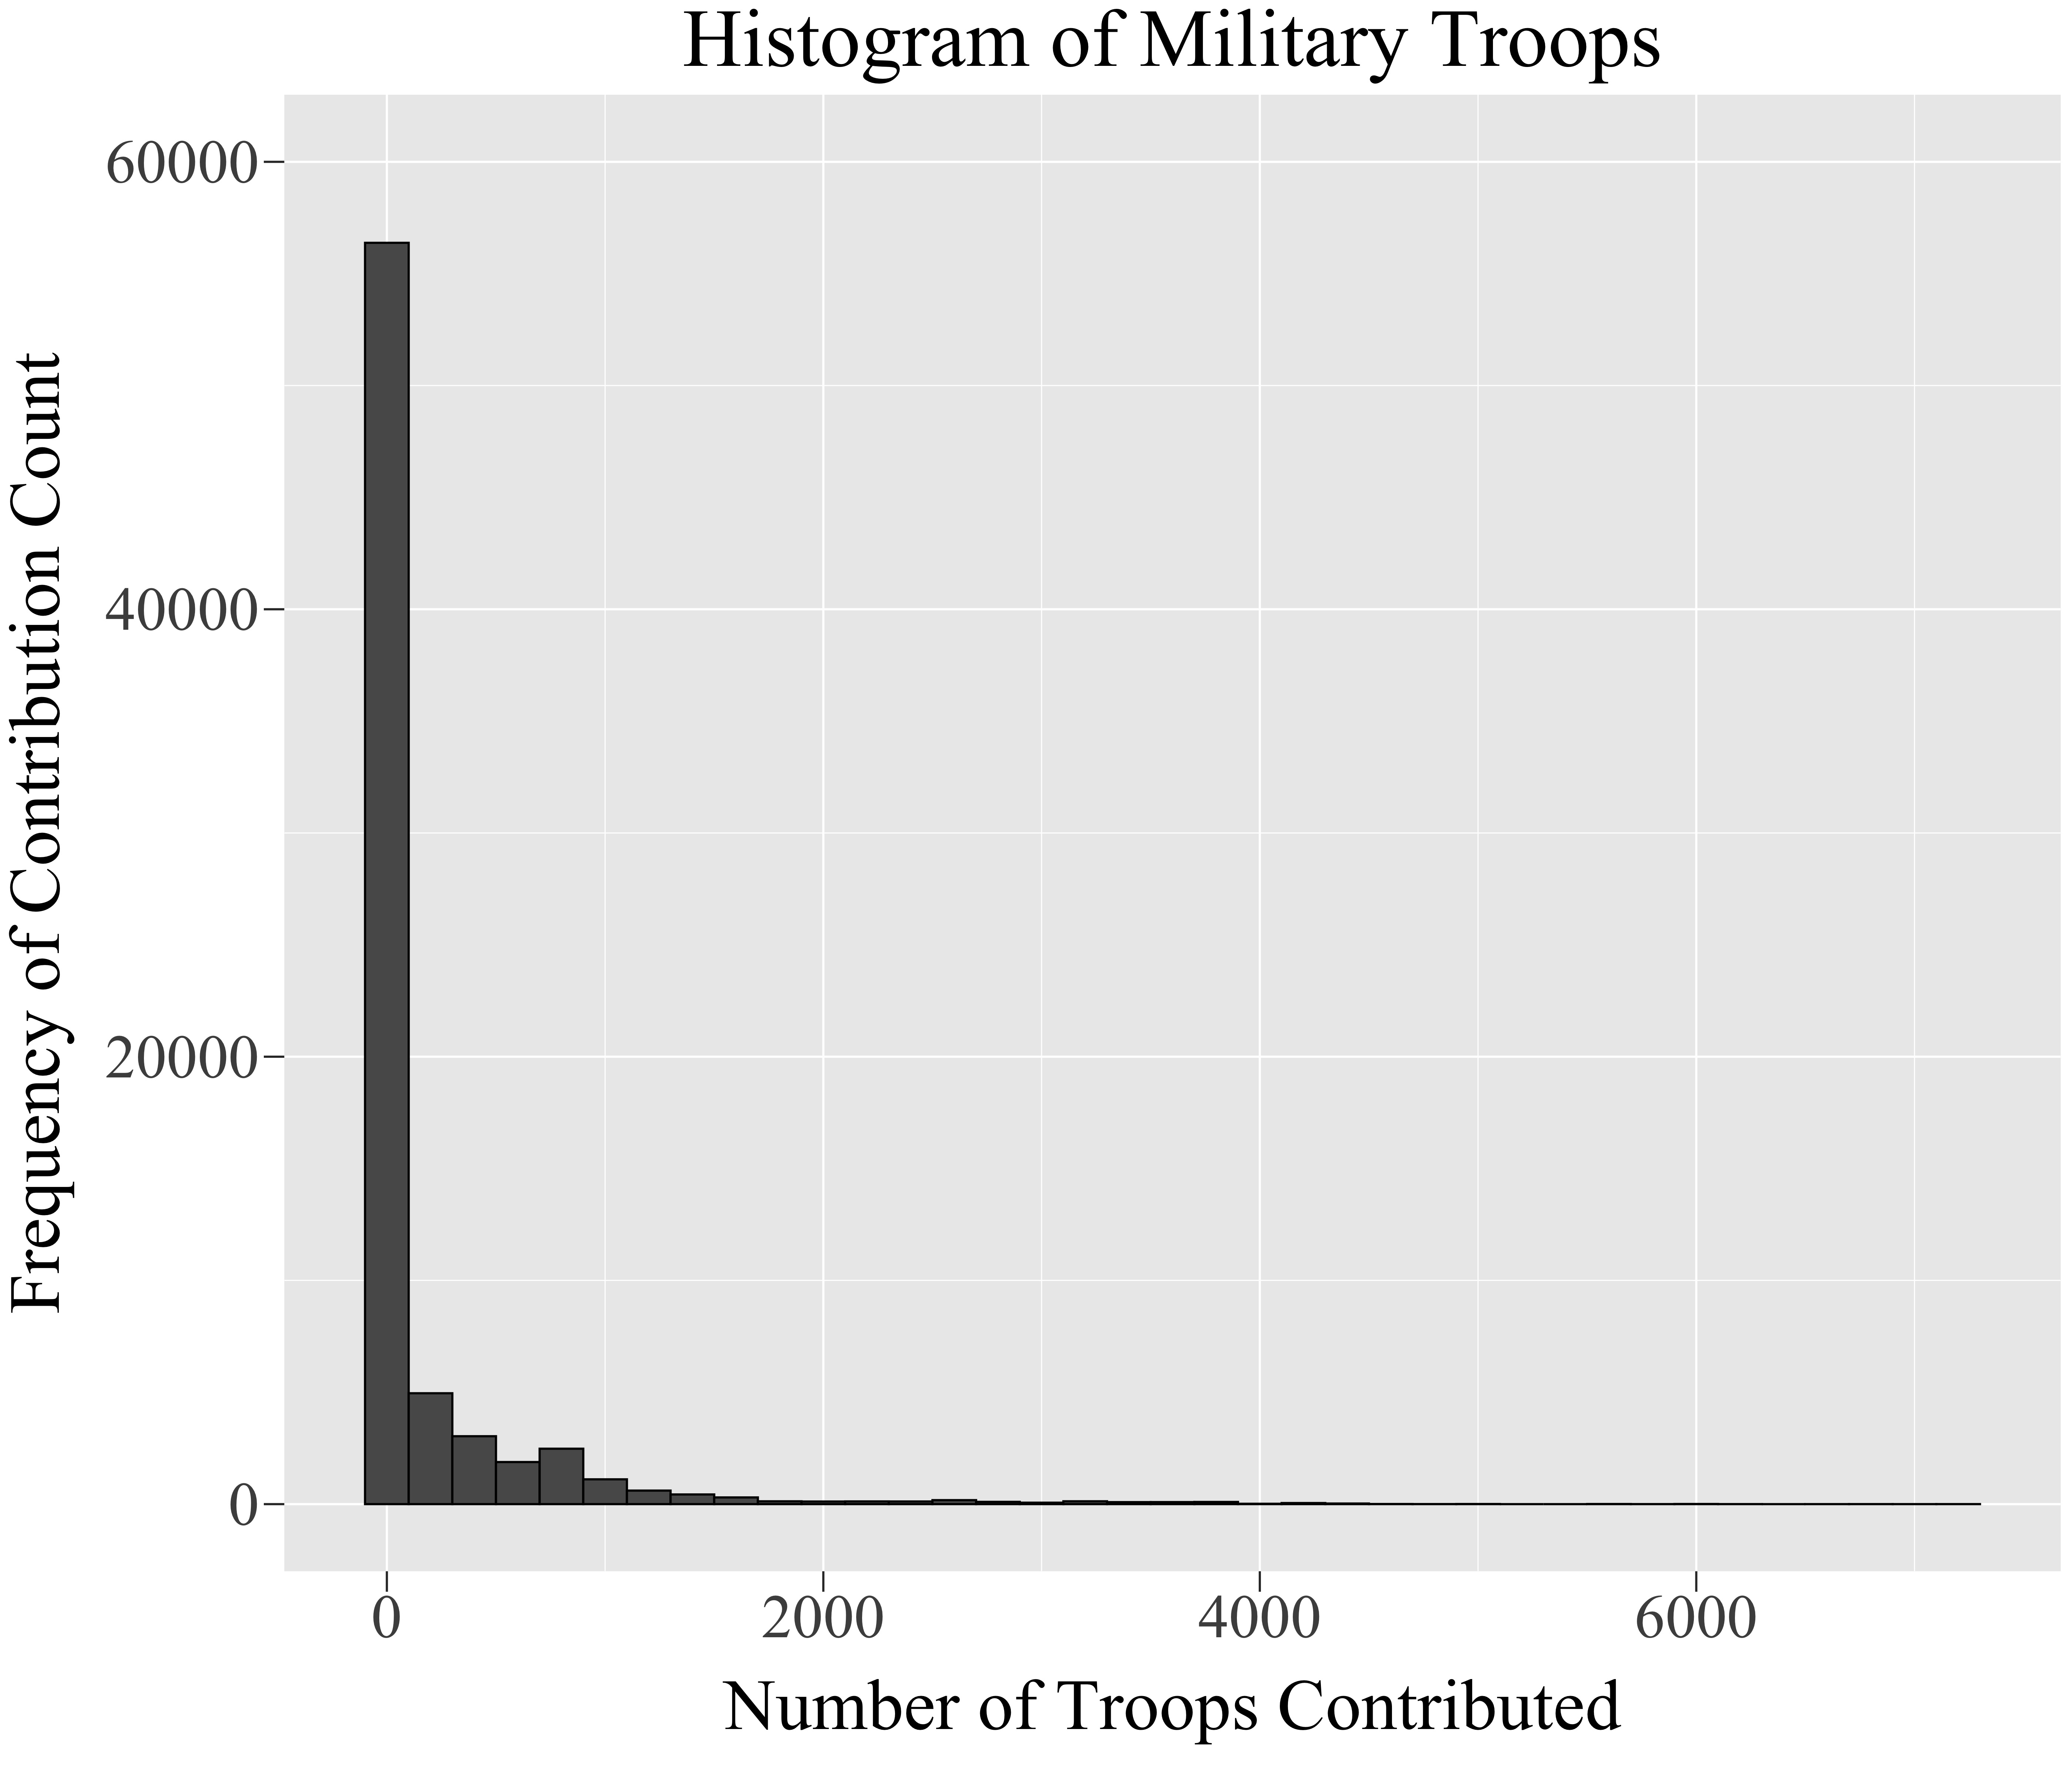
\includegraphics[width=\linewidth]{gg_Hist_DV_cont.jpg}
\caption{Histogram of Troops}
\end{subfigure}
\hfill
\begin{subfigure}[h]{0.5\linewidth}
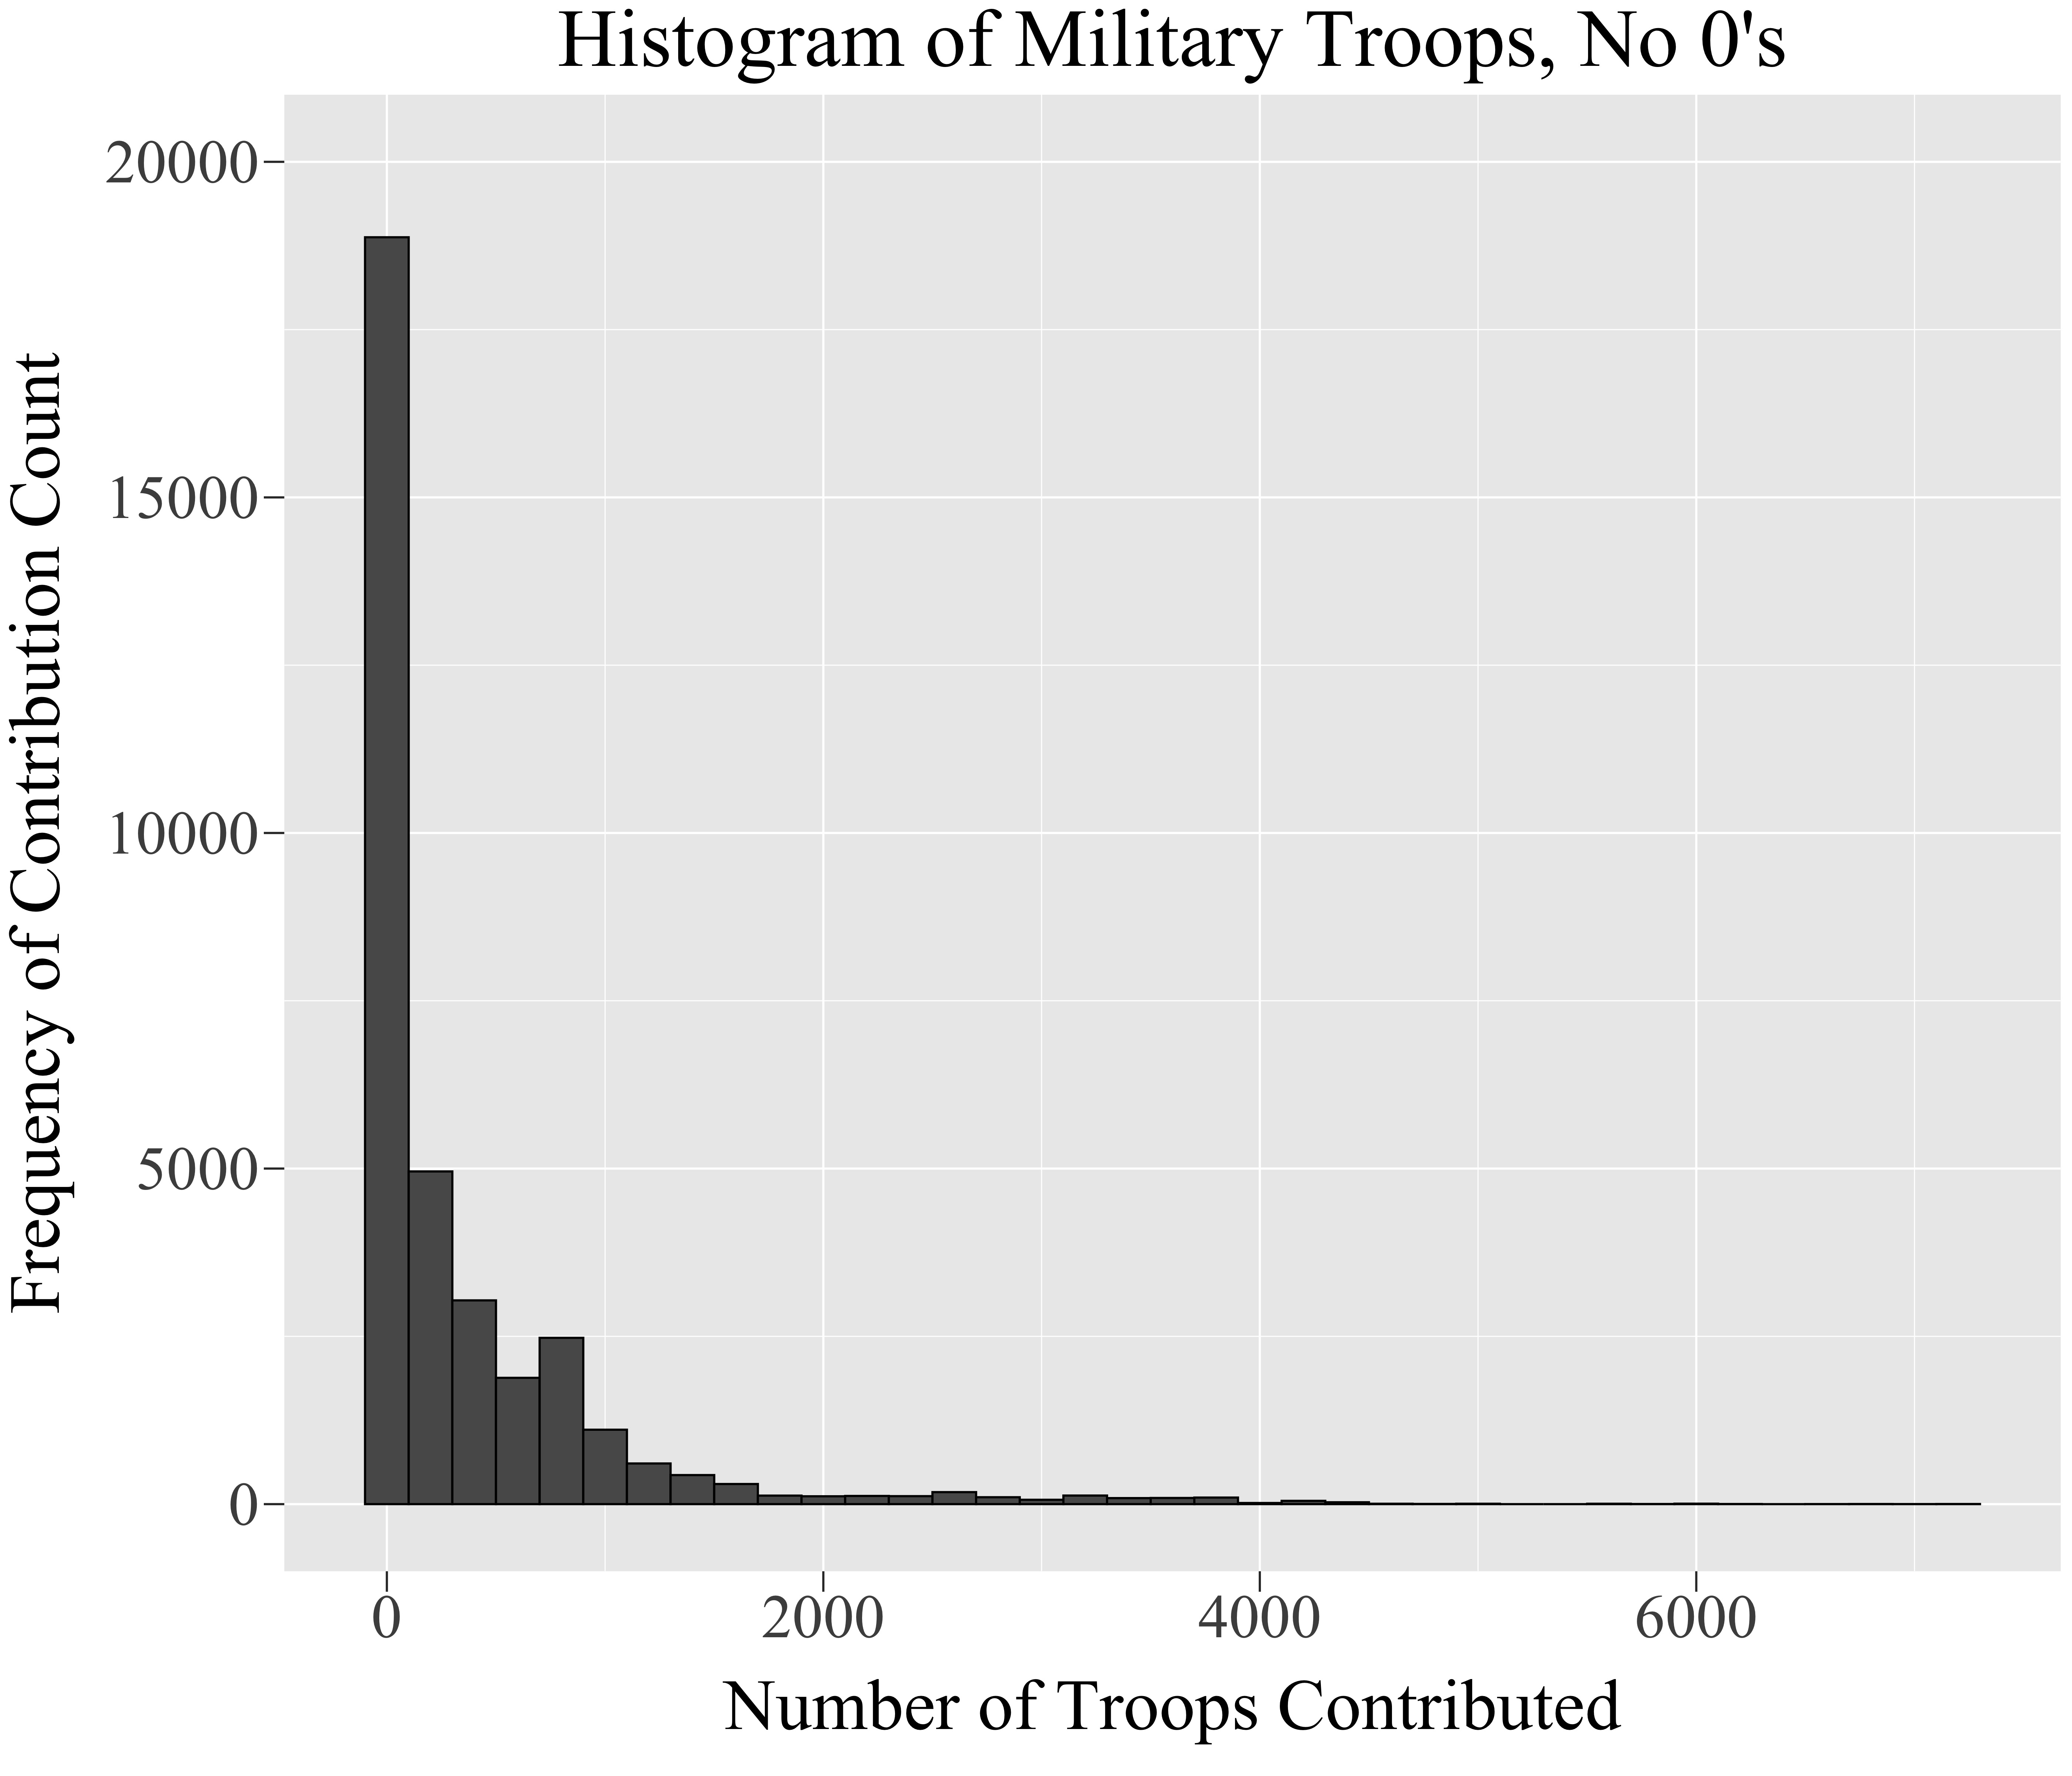
\includegraphics[width=\linewidth]{gg_Hist_DV_No_0_cont.jpg}
\caption{Histogram of Troops, No 0's}
\end{subfigure}%
\caption{\small Histograms of the troop contributions.}
% 12 words
\label{fig:Figure 1}
\end{figure}

While some scholars are interested in explaining mission shortfalls \citep[Ex.][]{passmore2018}, the theory of this project does not benefit from explaining shortfalls for two reasons. First, this project argues how mandate risk and conflict conditions signal information to individual contributors when making contributions, which demands a state-level unit of analysis. Collapsing to the mission-level unit of analysis would hide these state-based decisions that the theory explains. Second, the United Nations strategically sets troop authorizations to levels that minimize potential shortfalls. After the criticisms raised in the Brahimi Report \citep{Brahimi}, the United Nations has prioritized reducing mission shortfalls, as seen in Figure \ref{fig:LOESS}. The United Nations utilizes information gleaned from tactical assessments \citep{OMA}, state interactions within the organization \citep{joshi2020}, and Memoranda of Understanding negotiations to strategically set troop authorizations. As a result, troop authorization levels will be strategically reduced by the United Nations regardless of mandate risk leading to biased results in favor of smaller shortfalls. 
% 163 words

\subsection*{Independent Variables}

\begin{figure}[t!]
\begin{centering}
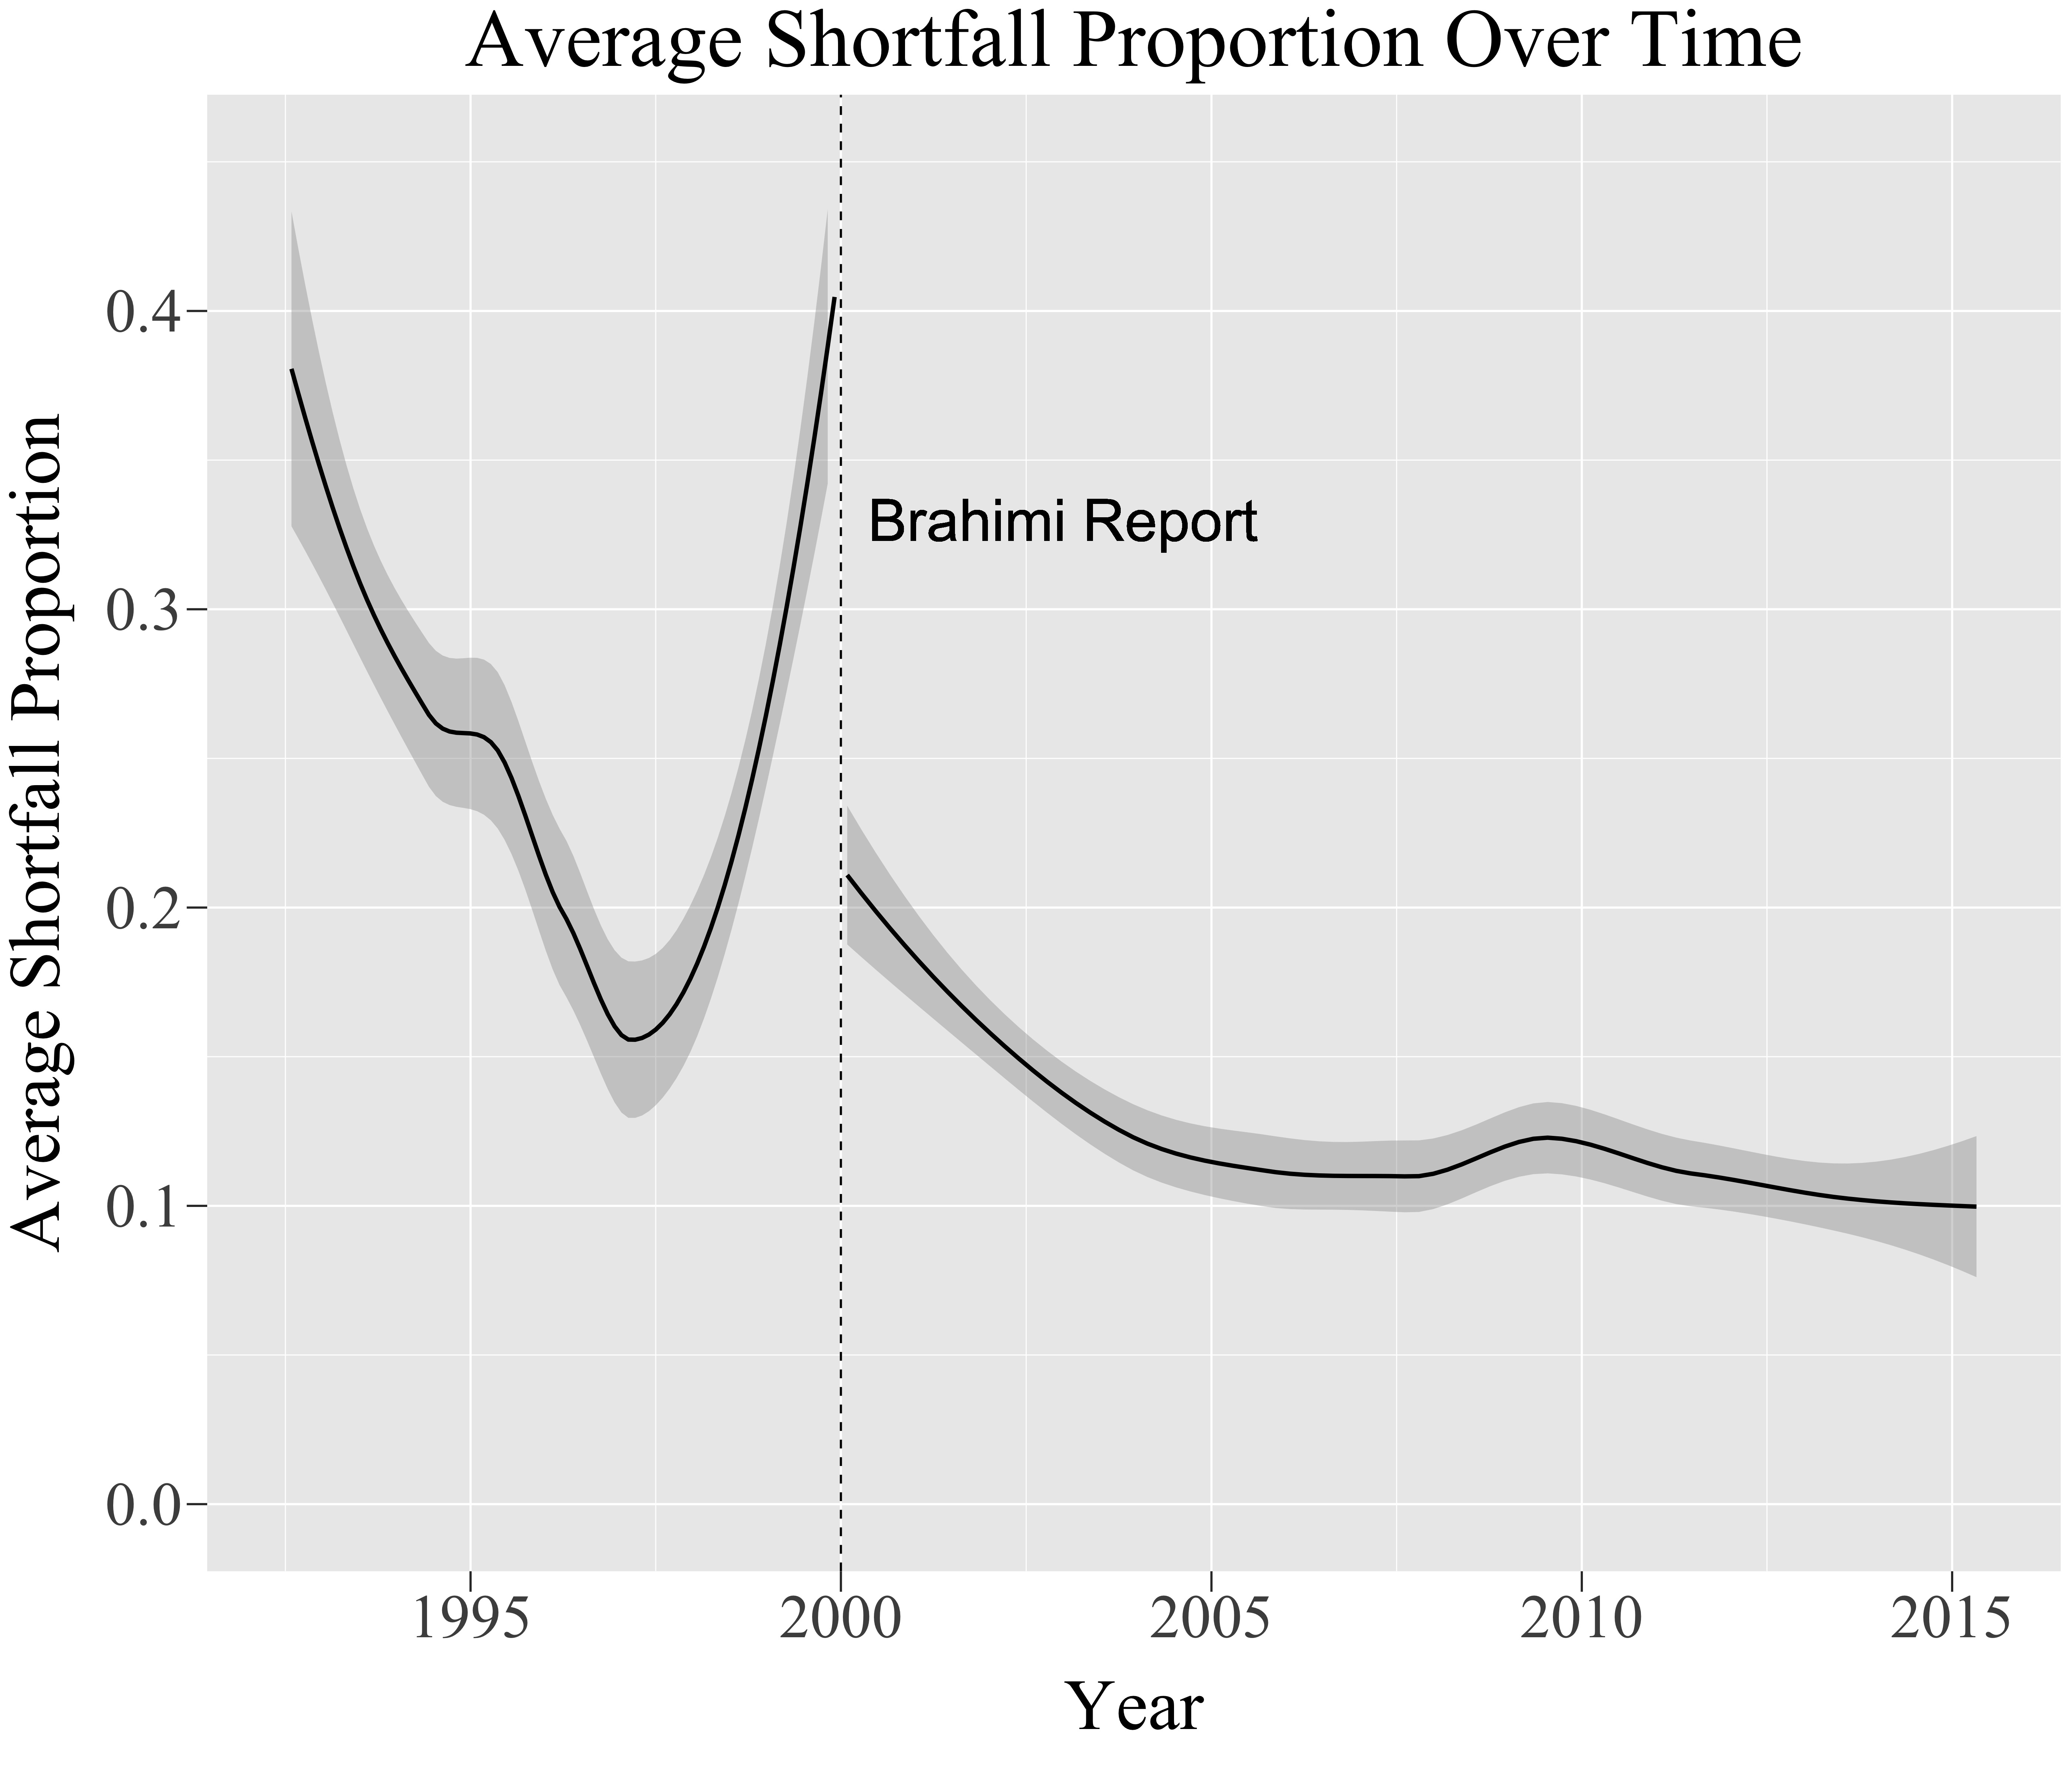
\includegraphics[width=100mm]{gg_shortfall_learning.jpg}
\caption{LOESS graph of mean shortfall proportion.}
\label{fig:LOESS}
\end{centering}
\end{figure}

I use the Tasks Assigned to Missions in their Mandates (TAMM) dataset to capture the tasks within peacekeeping mandates. The task categorization can be found in Table 1 with a richer classification explanation in Appendix E. This dataset developed by \cite{lloyd2021} covers all United Nations mission mandates from 1948-2015. Mandate tasks are time-variant and are coded at the mission-month level as mission mandates are often updated mid-mission. A task refers to any directive assigned to a mission in the mandate such as monitoring a ceasefire. Each mandate task is coded as a binary indicator where ``1'' indicates that the task is present in the mandate. 
% 106 words

To measure mandate risk, I develop a risk ratio index. Upon their creation, mission mandates contain several tasks that include risky and less risky tasks. When states make contributions, they observe risk as the aggregate of all risky tasks within the mission mandate. To capture this process, I create a risk ratio measure\footnotemark[10] based on the tasks found in Table 1. Per Equation \ref{equation 1}, I count the total number of risky tasks and divide it by the total number of mandate tasks. The variable is constrained from [0, 1]. 
% 89 words

\footnotetext[10]{\doublespacing \fontsize{12}{12}\selectfont The risk ratio measure does not place tasks on a risk continuum as it is difficult to imply an inherent ordering and distance between each task in terms of risk. For example, I can distinguish that Chapter VII enforcement is riskier than the promotion of press freedom, but it is difficult distinguish the difference in risk between buffer zone monitoring and Chapter VII enforcement. As a result, the proportion of risky tasks in the mandate is the best alternative to capturing mandate risk.}
% 83 words

\begin{equation}
	\textrm{Risk Ratio$_{t-1}$} = \frac{\sum \textrm{Risky Tasks$_{t-1}$}}{\sum \textrm{Total Tasks$_{t-1}$}}
	\label{equation 1}
\end{equation}
% 6 words

Battle deaths\footnotemark[11] capture the conflict environment difficulty that states consider when contributing troops. The battle death data comes from the UCDP Geo-referenced Event Dataset \citep{sundberg2013}. I use the monthly summation of the total number of deaths due to conflict, which includes battle deaths and civilian killings. I include the interaction of risk ratio and total battle deaths to test hypothesis 2.\footnotemark[12]
% 65 words

\footnotetext[11]{\doublespacing \fontsize{12}{12}\selectfont Scholars find that contributors reduce their contributions in response to peacekeeper fatalities \citep[Ex.][]{oestman2021price}. I include total and malicious peacekeeper fatalities that a contributor and the mission experiences from \cite{henke2019} and find no statistical significance nor increased model fit for a one, three, or six month lag. As a result, I do not include fatalities in the models.}
% 760words

\footnotetext[12]{\doublespacing \fontsize{12}{12}\selectfont Some argue that mandate risk is endogenous to conflict conditions as difficult conflict environments would foster risky mandates. If this is true, the effect of mandate risk on contributions would be spurious. To ensure that mandate risk is not spurious to a difficult conflict environment, I employ a fractional logistic model where battle deaths and mission-level variables predict risk ratio. I find that battle deaths do not affect mandate risk meaning mandate risk has an independent effect on troop contributions. The results can be found in Appendix D.}
% 89 words

In a secondary analysis, I disaggregate risk ratio into individual risky tasks. I evaluate each risky task by interacting the task with battle deaths and plotting each task individually at various levels of battle deaths to investigate the task's marginal effect on troop contributions. This disaggregation further probes how mandate tasks deter troop contributions while also providing corroborating evidence to the main analysis. 
% 63 words

\subsection*{Controls}

To remove potential confounding effects, the model includes groups of control variables drawn from the literature. The controls are divided into mission, contributor, and dyad controls. Mission level controls\footnotemark[13] account for other mission-specific characteristics. I include the number of contributors in each mission month from the International Peace Institute's Peacekeeping Database \cite{perry2013} to capture the collective action problem regarding troop provisions. From \cite{koops2015oxford}, I code whether the mission was ``re-hatted'' or was a previous United Nations mission. To ensure that mandate risk is not spurious to mission shortfalls, I include the difference between the number of authorized troops and the total number of contributed troops in a mission month \citep{passmore2018}. Due to data limitations, the main models will be those without the shortfall variable making shortfalls function as a robustness check. 
% 140 words

\footnotetext[13]{\doublespacing \fontsize{12}{12}\selectfont Some argue that host state characteristics of the number of discriminated groups \citep{vogt2015integrating} and rugged terrain \citep{shaver2019terrain} affect contributions; however, I do not include these variables due to a lack of statistical significance nor improved model fit.}
% 43 words

The second group of controls accounts for a state's propensity to contribute troops. I include the contributor's gross domestic product per capita from the United Nations' Department of Statistics \citep{UN_GDP} and the contributor's level of democracy from the Varieties of Democracy dataset's polyarchy variable \citep{VDemV11} to capture the effects of wealth and regime type on a state's propensity to contribute. The model also contains the total number of troops that a contributor deployed to all peacekeeping operations \citep{perry2013}. Last, I include the proportion of a state's military personnel that is deployed to a specific mission each month with the count of military personnel coming from the Correlates of War National Material Capabilities dataset (v6.0) \citep{CINC}. 
% 128 words

The last group of controls incorporates the relationship between the potential contributor and the host state. I create an indicator of whether the host and contributor are on the same continent since neighboring\footnotemark[14] states are likely to contribute troops to stop conflict contagion. The model also includes the level of bilateral trade \citep{barbieri2009trading} and the number of joint international organization memberships \citep{pevehouse2020tracking} to include the level of international connection between the two states. 
% 79 words

\footnotetext[14]{\doublespacing \fontsize{12}{12}\selectfont I employ the Correlates of War Project Direct Contiguity dataset \citep{stinnett2002correlates} to investigate if contiguous states send more peacekeepers. A Wald test demonstrates that contiguity is not distinguishable from zero nor adds to model fit.}
% 38 words

\subsection*{Method}

I use the negative binomial estimator due to the over dispersion of the dependent variable. To combat heteroskedasticity and auto-correlation, I cluster the error term on the contributing country and include a lagged dependent variable as a regressor. I lag each independent variable by one month to ensure the ordering of the treatment and outcome. To demonstrate the robustness of the results, I provide multiple alternative specifications. First, I include observations with more than 200 battle deaths. Second, I include observer missions in the sample. Third, I expand the potential contributor sample to include 30 randomly selected non-contribution states. Fourth, I employ a sample of major powers and contributors on the same continent as the mission host state \citep{Crescenzi2011}. Fifth, I include a sample of only states who ever contributed to a mission. Last, I employ a zero-inflated negative binomial estimator. Each alternative specification presents results consistent with the main analysis and can be found in Appendix A. In Appendix C, I replicate the 15 and 30 potential contributor sampling procedure to generate ten samples for both counts. I employ meta-analysis to estimate an overall average of the effects across the 10 samples for the 15 and 30 potential contributor sample to demonstrate that the results are not an artifact of the sampling procedure. 
% 217 words

\section*{Results}

\begin{table}[htbp]\centering
\footnotesize
\def\sym#1{\ifmmode^{#1}\else\(^{#1}\)\fi}
\caption{The Effect of Risk Ratio on Contributions \label{Table 2}}
\begin{tabular}{l*{5}{c}}
\hline\hline
                    &\multicolumn{1}{c}{Model 1} &\multicolumn{1}{c}{Model 2} &\multicolumn{1}{c}{Model 3} &\multicolumn{1}{c}{Model 4} &\multicolumn{1}{c}{Model 5}        \\
\hline
Risk Ratio$_{t-1}$          &      -1.601\sym{**}&      -2.103\sym{**}&      -1.875\sym{**}&      -1.250\sym{**}&      -1.179\sym{**}\\
                    &     (0.498)        &     (0.459)        &     (0.477)        &     (0.444)        &     (0.457)        \\
[0.5em]
Battle Deaths$_{t-1}$ (Hundreds)&       0.012        &       0.072        &       2.359\sym{**}&       0.087        &       0.929        \\
                    &     (0.085)        &     (0.099)        &     (0.636)        &     (0.104)        &     (0.668)        \\
Risk Ratio$_{t-1}$ X Battle Deaths$_{t-1}$&                    &                    &      -3.086\sym{**}&                    &      -1.150        \\
                    &                    &                    &     (0.858)        &                    &     (0.940)        \\
[0.5em]
Troop Shortfall$_{t-1}$ (Hundreds)&                    &                    &                    &       0.015\sym{**}&       0.015\sym{**}\\
                    &                    &                    &                    &     (0.002)        &     (0.002)        \\
[0.5em]
Number of Contributors$_{t-1}$ (Tens)&                    &      -0.069\sym{\dagger} &      -0.073\sym{\dagger} &      -0.099\sym{**}&      -0.100\sym{**}\\
                    &                    &     (0.036)        &     (0.038)        &     (0.038)        &     (0.038)        \\
[0.5em]
Re-hatted$_{t-1}$           &                    &      -0.045        &      -0.043        &      -0.131        &      -0.130        \\
                    &                    &     (0.156)        &     (0.155)        &     (0.169)        &     (0.169)        \\
[0.5em]
Previous UN Mission$_{t-1}$ &                    &       0.555\sym{**}&       0.539\sym{**}&       0.486\sym{**}&       0.479\sym{**}\\
                    &                    &     (0.132)        &     (0.133)        &     (0.156)        &     (0.156)        \\
[0.5em]
Contributor GDP per Capita$_{t-1}$ (Ten Thousands)&                    &      -0.114\sym{*} &      -0.114\sym{*} &      -0.110\sym{*} &      -0.110\sym{*} \\
                    &                    &     (0.053)        &     (0.052)        &     (0.050)        &     (0.050)        \\
[0.5em]
Contributor Democracy$_{t-1}$&                    &       2.324\sym{**}&       2.290\sym{**}&       2.315\sym{**}&       2.304\sym{**}\\
                    &                    &     (0.501)        &     (0.500)        &     (0.512)        &     (0.513)        \\
[0.5em]
Total Contributed Troops$_{t-1}$ (Hundreds)&                    &       0.027\sym{**}&       0.026\sym{**}&       0.020\sym{**}&       0.020\sym{**}\\
                    &                    &     (0.009)        &     (0.009)        &     (0.007)        &     (0.007)        \\
[0.5em]
Proportion of Contributor Troops$_{t-1}$&                    &       1.109\sym{\dagger} &       1.108\sym{\dagger} &       1.462\sym{\dagger} &       1.459\sym{\dagger} \\
                    &                    &     (0.576)        &     (0.575)        &     (0.773)        &     (0.771)        \\
[0.5em]
Same Continent$_{t-1}$      &                    &      -0.004        &       0.005        &      -0.160        &      -0.155        \\
                    &                    &     (0.170)        &     (0.166)        &     (0.176)        &     (0.174)        \\
[0.5em]
Trade$_{t-1}$ (Billions)    &                    &       0.168\sym{*} &       0.162\sym{*} &       0.314\sym{**}&       0.310\sym{**}\\
                    &                    &     (0.080)        &     (0.076)        &     (0.118)        &     (0.117)        \\
[0.5em]
Joint IOs$_{t-1}$           &                    &       0.020\sym{**}&       0.019\sym{**}&       0.020\sym{**}&       0.020\sym{**}\\
                    &                    &     (0.007)        &     (0.007)        &     (0.007)        &     (0.007)        \\
[0.5em]
Troops$_{t-1}$              &       0.632\sym{**}&       0.519\sym{**}&       0.519\sym{**}&       0.551\sym{**}&       0.550\sym{**}\\
                    &     (0.093)        &     (0.083)        &     (0.083)        &     (0.092)        &     (0.092)        \\
[0.5em]
Constant            &       3.529\sym{**}&       1.833\sym{**}&       1.707\sym{**}&       0.987        &       0.953        \\
                    &     (0.430)        &     (0.604)        &     (0.602)        &     (0.627)        &     (0.623)        \\
\hline
lnalpha             &       2.056\sym{**}&       1.884\sym{**}&       1.882\sym{**}&       1.753\sym{**}&       1.752\sym{**}\\
                    &     (0.099)        &     (0.090)        &     (0.090)        &     (0.089)        &     (0.089)        \\
\hline
Observations        &       78659        &       72553        &       72553        &       61665        &       61665        \\
\hline\hline
\multicolumn{6}{l}{\footnotesize State clustered standard errors in parentheses}\\
\multicolumn{6}{l}{\footnotesize Dependent variable is troop counts. 15 potential contributor random sample.}\\
\multicolumn{6}{l}{\footnotesize \sym{\dagger} \(p<0.10\), \sym{*} \(p<0.05\), \sym{**} \(p<0.01\). Two-tailed test.}\\
\end{tabular}
\end{table}

% 228 words

Hypothesis 1 states that as the mandate risk ratio increases, the number of contributed troops will decrease. Table 2 provides strong support for the first hypothesis. In a naïve approach, Model 1 demonstrates that risk ratio is negatively associated with troop contributions at \textit{p $<$ 0.01}. Moving to Model 2 with the full list of controls, mandate risk remains negative and statistically significant at \textit{p $<$ 0.01}. As a harder test, Model 4, which includes troop shortfalls, mandate risk is negative and statistically significant at \textit{p $<$ 0.01}. For substantive significance, Figure \ref{fig:RR} presents predicted troop contributions across values of mandate risk with all other variables held at their central tendencies. For Model 2, a min to max shift of mandate risk from 0.40 to 1 reduces the predicted contribution from 53 to 15 troops, which is a 72\% reduction. In more substantive terms, the average number of contributors in the sample is 15 per mission month. Missions with a risk ratio of 0.4 will have about 795 troops in a month while a mission with a risk ratio of 1 will have about 225 troops in a month, on average. As a harder test, a min to max shift of mandate risk for Model 4 represents a 53\% reduction from 40 to 19 troops. 
% 215 words

As further evidence, I draw on two missions: the United Nations Interim Force in Lebanon (UNIFIL) with an authorization of about 6,000 troops and the United Nations Transitional Administration for Eastern Slavonia, Baranja, and Western Sirmium (UNTAES) with an authorization of about 5,000 troops. In 1997, UNIFIL had a risk ratio of 0.5 suggesting an equal amount of risky and less risky tasks and maintained an average troop contribution of 478 troops when a state decided to contribute. In contrast, UNTAES in 1997 had a risk ratio of 1 and an average troop contribution of 298 when a state decided to contribute. This means that UNTAES had a 37\% smaller average contribution than UNIFIL when it maintained a twice as risky mandate. This provides further evidence that risky missions receive decreased troop contributions supporting Hypothesis 1.
% 136 words

\begin{figure}[t!]
\begin{subfigure}[h]{0.5\linewidth}
\includegraphics[width=\linewidth]{gg_M2_sim.jpg}
%\caption{Histogram of Troops}
\end{subfigure}
\hfill
\begin{subfigure}[h]{0.5\linewidth}
\includegraphics[width=\linewidth]{gg_M4_sim.jpg}
%\caption{Histogram of Troops, No 0's}
\end{subfigure}
\vspace{-3mm}
\caption{\small Predicted troop contributions with 95\% confidence intervals for Models 2 (left) and 4 (right).}
% 14 words
\label{fig:RR}
\end{figure}

After finding support for Hypothesis 1, I turn to evaluate Hypothesis 2 that states that the negative effect of mandate risk on troop contributions will strengthen as the number of battle deaths increase. In Models 3 and 5, the constituent term of risk ratio is negative and significant at \textit{p $<$ 0.01} signifying that when monthly battle deaths are at zero, mandate risk reduces troop contributions. For Model 3, the constituent term of battle deaths is positive and significant at \textit{p $<$ 0.01}, meaning when risk ratio is equal to zero, battle deaths increase troop contributions, but a risk ratio of zero does not exist in this sample. Furthermore, in Model 3, the interaction of risk ratio and battle deaths is negative and significant at \textit{p $<$ 0.01}, but Model 5's interaction is not significant; however interaction term significance is best evaluated by a graph. Based on Figure \ref{fig:RR_X_bd}, the interaction terms in Models 3 and 5 are negative significant at \textit{p $<$ 0.05} across all levels of battle deaths, except for Model 5 when battle deaths near 200. For Model 3, a min to max shift of battle deaths from zero to 200 represents a marginal effect increase from negative 39 troops to about negative 154 troops. For the harder test of Model 5, a min to max shift of battle deaths is an increase from negative 28 troops to negative 91 troops. These substantive effects provide strong evidence in support of Hypothesis 2 that the effect of risky mandates becomes increasingly strong as the conflict becomes more dangerous. 
% 260 words

\begin{figure}[t!]
\begin{subfigure}[h]{0.5\linewidth}
\includegraphics[width=\linewidth]{gg_M3_sim.jpg}
%\caption{Histogram of Troops}
\end{subfigure}
\hfill
\begin{subfigure}[h]{0.5\linewidth}
\includegraphics[width=\linewidth]{gg_M5_sim.jpg}
%\caption{Histogram of Troops, No 0's}
\end{subfigure}
\vspace{-3mm}
\caption{\small Marginal effect of risk ratio on contributions conditional on battle deaths with 95\% confidence intervals from Models 3 (left) and 5 (right).}
% 24 words
\label{fig:RR_X_bd}
\end{figure}

A few control variables present interesting relationships. Increased shortfalls and missions that are a continuation, such as UNOSOM moving to UNOSOM II, are associated with higher contributions. Due to collective action problems, more contributors reduce the number of troops states deploy. While richer states send fewer troops, democratic states make larger contributions, which is counter to the literature \citep[Ex.][]{duursma2019}. States who send a larger proportion of their armed forces and are large contributors send larger deployments. States who trade more and maintain more international organization relationships with the host state contribute more troops.
% 97 words

\section*{Disaggregation of Risk Ratio}

After finding support for both theoretical implications, I now investigate the effect of individual risky tasks on troop contributions. For this analysis, I estimate individual models for the interaction of each risky task with battle deaths to capture state decisions in light of the task and conflict environment. The goal of this analysis is to probe each task's direction with respect to contributions. Figure \ref{fig:Tasks} visualizes the marginal effect of the task on contributions conditional on battle deaths at zero, its mean, and one standard deviation above the mean with control variables at their central tendencies. The analysis provides rough evidence of each task's respective influence on contributions. 
% 108 words

Figure \ref{fig:Tasks} presents a few interesting patterns. First, some tasks, while exhibiting a positive marginal effect, demonstrate diminishing positive effects, such as the agreement implementation, humanitarian protection, and United Nations personnel protection tasks. Second, other tasks signal contributor willingness to accept risky actions, as seen by security and police reform assistance and refugee assistance. Overall, risky tasks demonstrate both deterring and compelling effects on contributions conditional on battle deaths. While states make contribution decisions based on mandates as a whole, these estimates provide an initial investigation of which tasks may be driving the results found in the main analysis. 
% 99 words

\begin{figure}[t!]
\begin{subfigure}[h]{0.5\linewidth}
\includegraphics[width=\linewidth]{gg_Tasks_sim_1.jpg}
%\caption{Histogram of Troops}
\end{subfigure}
\hfill
\begin{subfigure}[h]{0.5\linewidth}
\includegraphics[width=\linewidth]{gg_Tasks_sim_2.jpg}
%\caption{Histogram of Troops, No 0's}
\end{subfigure}
\vspace{-5mm}
\caption{\small Marginal Effect of Risky Tasks on Troops Contributions}
% 8 words
\label{fig:Tasks}
\end{figure}

\section*{Note on Endogeneity}

It is common for peacekeeping statistical models to suffer from endogeneity \citep[Ex.][]{fortna2004,beardsley2011,fjelde2019}, but like past studies, I argue that endogeneity biases against my findings. Peacekeeping missions are not randomly assigned since mission authorization is contingent on an unobserved factor, the United Nations decision-making process. To avoid building a poor reputation, the United Nations is incentivized to provide the mission with sufficient resources to successfully implement the mandate leading the United Nations to campaign for larger contributions. In addition, the United Nations will authorize the mission with more risky tasks to support the mission's goal of peace generation, such as when the United Nations authorized the use of force to protect civilians in Libya \citep{Civs_Libya}. Due to the dual positive correlations between the unobserved factor, mandate risk, and troop contributions, the overall bias is positive thereby under-estimating the results. 
% 148 words

Another source of bias concerns the optimal level of troops required to fulfill each task. The United Nations does not provide guidelines concerning the number of troops required for each task. However, mission force commanders are instructed to deploy larger troop contingents as a costly signal of resolve to deter future violence \citep{fearon1997signaling,Infantry}. To effectively deter future conflict, the mission needs more risky tasks that authorize the use of force. The dual positive correlation between optimal troop levels, mandate risk, and troop contributions creates a positive bias that under-reports the results. 
% 97 words

\section*{Conclusion}

This study explains how mission mandates and the conflict environment affects troop contributions to United Nations peacekeeping missions. The peacekeeping contribution literature has overlooked critical mission-specific characteristics that affect contribution decisions, specifically mission mandates and the conflict environment. Using regression analysis, I find that risky mandates reduce troop contributions to peacekeeping missions, especially when the conflict environment becomes increasingly dangerous. The disaggregation of mandate risk demonstrates that some risky tasks deter contributions while others entice deployments. Overall, I find that states reduce their respective troop contributions when mandates are increasingly risky and when the conflict environment is dangerous suggesting that while the United Nations prefers to intervene in the hardest conflicts, states prefer the relatively easy ones.  
% 117 words

This study provides major implications for those investigating peacekeeping effectiveness and the effects of mission size \citep[Ex.][]{hultman2013united,fjelde2019,phayal2020}. This study suggests that larger peacekeeping missions are most likely a product of less risky mandates and safe conflict environments. Missions with risky mandates and dangerous conflict environments limit the generation of large mission sizes, hindering conflict-related outcomes. Furthermore, the United Nations' reliance on Chapter VII authorization and civilian protection mandates \citep{Prot_Civs} is inadvertently reducing troop contributions to the most difficult missions limiting mission effectiveness. Policymakers must note the unintended consequences of the Responsibility to Protect and the foundation of civilian protection mandates while expanding the use of risk premiums to attract contributors \citep{razza_2020}. Increasing the employment of risk premiums in risky missions should increase contributor benefits and entice contributions. 
% 142 words

Future studies should further consider how mission mandates affect the benefits required to maintain contributors throughout the mission as well as the duration of peace after risky mandated missions. This study demonstrates that states gather information from mandates and the mission conditions that signal the likelihood of losing troops on mission. To overcome these costs, pivotal states likely need to further increase foreign aid to supply the mission \citep{boutton2020}. Second, missions with risky mandates are likely to be under-supplied and ineffective. As a result, risky mandated missions are unlikely to create conditions that lead to long-term peace once the mission leaves.
% 104 words

\newpage

%%%% Tables for paper since you have to say "table" or "figure" about here. %%%%

%%% Task Table %%%%

%\begin{singlespace}
%\begin{table}[t]\centering
\fontsize{7.5}{7.5}\selectfont
\def\sym#1{\ifmmode^{#1}\else\(^{#1}\)\fi}
\caption{Table of Task Risk}
\label{Table 1}
\begin{tabular}{c*{2}{c}}
\hline\hline
                    \multicolumn{1}{c}{Risky}         &\multicolumn{1}{c}{Less Risky}      \\
\hline \\
Monitor Peace Agreements                                & Promote Good Offices (Subtask of Monitor Peace Agreements) \\
Subtasks: Buffer Monitor and Liaise War Parties         &  \\
[0.5em]
Monitor Human Rights                                    &   Monitor the Weapons Trade, Monitor Weapons Embargo, \\ 
Subtask: Monitor the Refugee Situation                  & Inspect Cargo (Subtasks of Monitor Borders) \\ 
[0.5em]
Protect Human Rights                                    & Monitor Use of Natural Resources \\
Subtasks: Protect Children, Protect Women,              &  \\
Protect Civilians                                       & \\
[0.5em]
Protect UN Personnel (Ensure Security)                  & Monitor Elections \\
[0.5em]
Assist in Demining                                     & Provide Security During the Electoral Period\\     
[0.5em]
Monitor Borders                                         & Assist with Election Implementation \\
                                                        & (Technical or Logistical Assistance) \\
[0.5em]
Chapter VII Authorization                               & Build Government Capacity \\
                                                        & Subtask: Implement Government Policies \\
[0.5em]
Assist with Security Sector Reform                      & Preserve Cultural and Historical Sites \\ 
Subtasks: Assist Police Reform, Monitor the Police,     &   \\
Conduct Joint Patrols with Police                        &   \\ 
[0.5em]
Monitor Disarmament, Demobilization,                    & Assist in the Implementation of Quick Impact Projects (QIP) \\
 and Reintegration                                      & \\
[0.5em]
Help Implement Disarmament, Demobilization,             & Assist with Justice Sector Reform \\ 
and Reintegration                                       & \\
[0.5em]
                                                        & Promote National Reconciliation \\
                                                        & Subtask: Pursue Justice for War Criminals \\
[0.5em]
                                                        & Disseminate Info About the Mission to the Public \\
[0.5em]
                                                        & Promote Freedom of the Press \\                                                                            
\hline\hline
\multicolumn{1}{l}{\footnotesize Table adapted from tasks coded in Lloyd (2021).}\\
\end{tabular}
\end{table}


%\end{singlespace}

\clearpage

%%% DV histograms %%%

\begin{comment}
\begin{figure}[t!]
\begin{subfigure}[h]{0.5\linewidth}
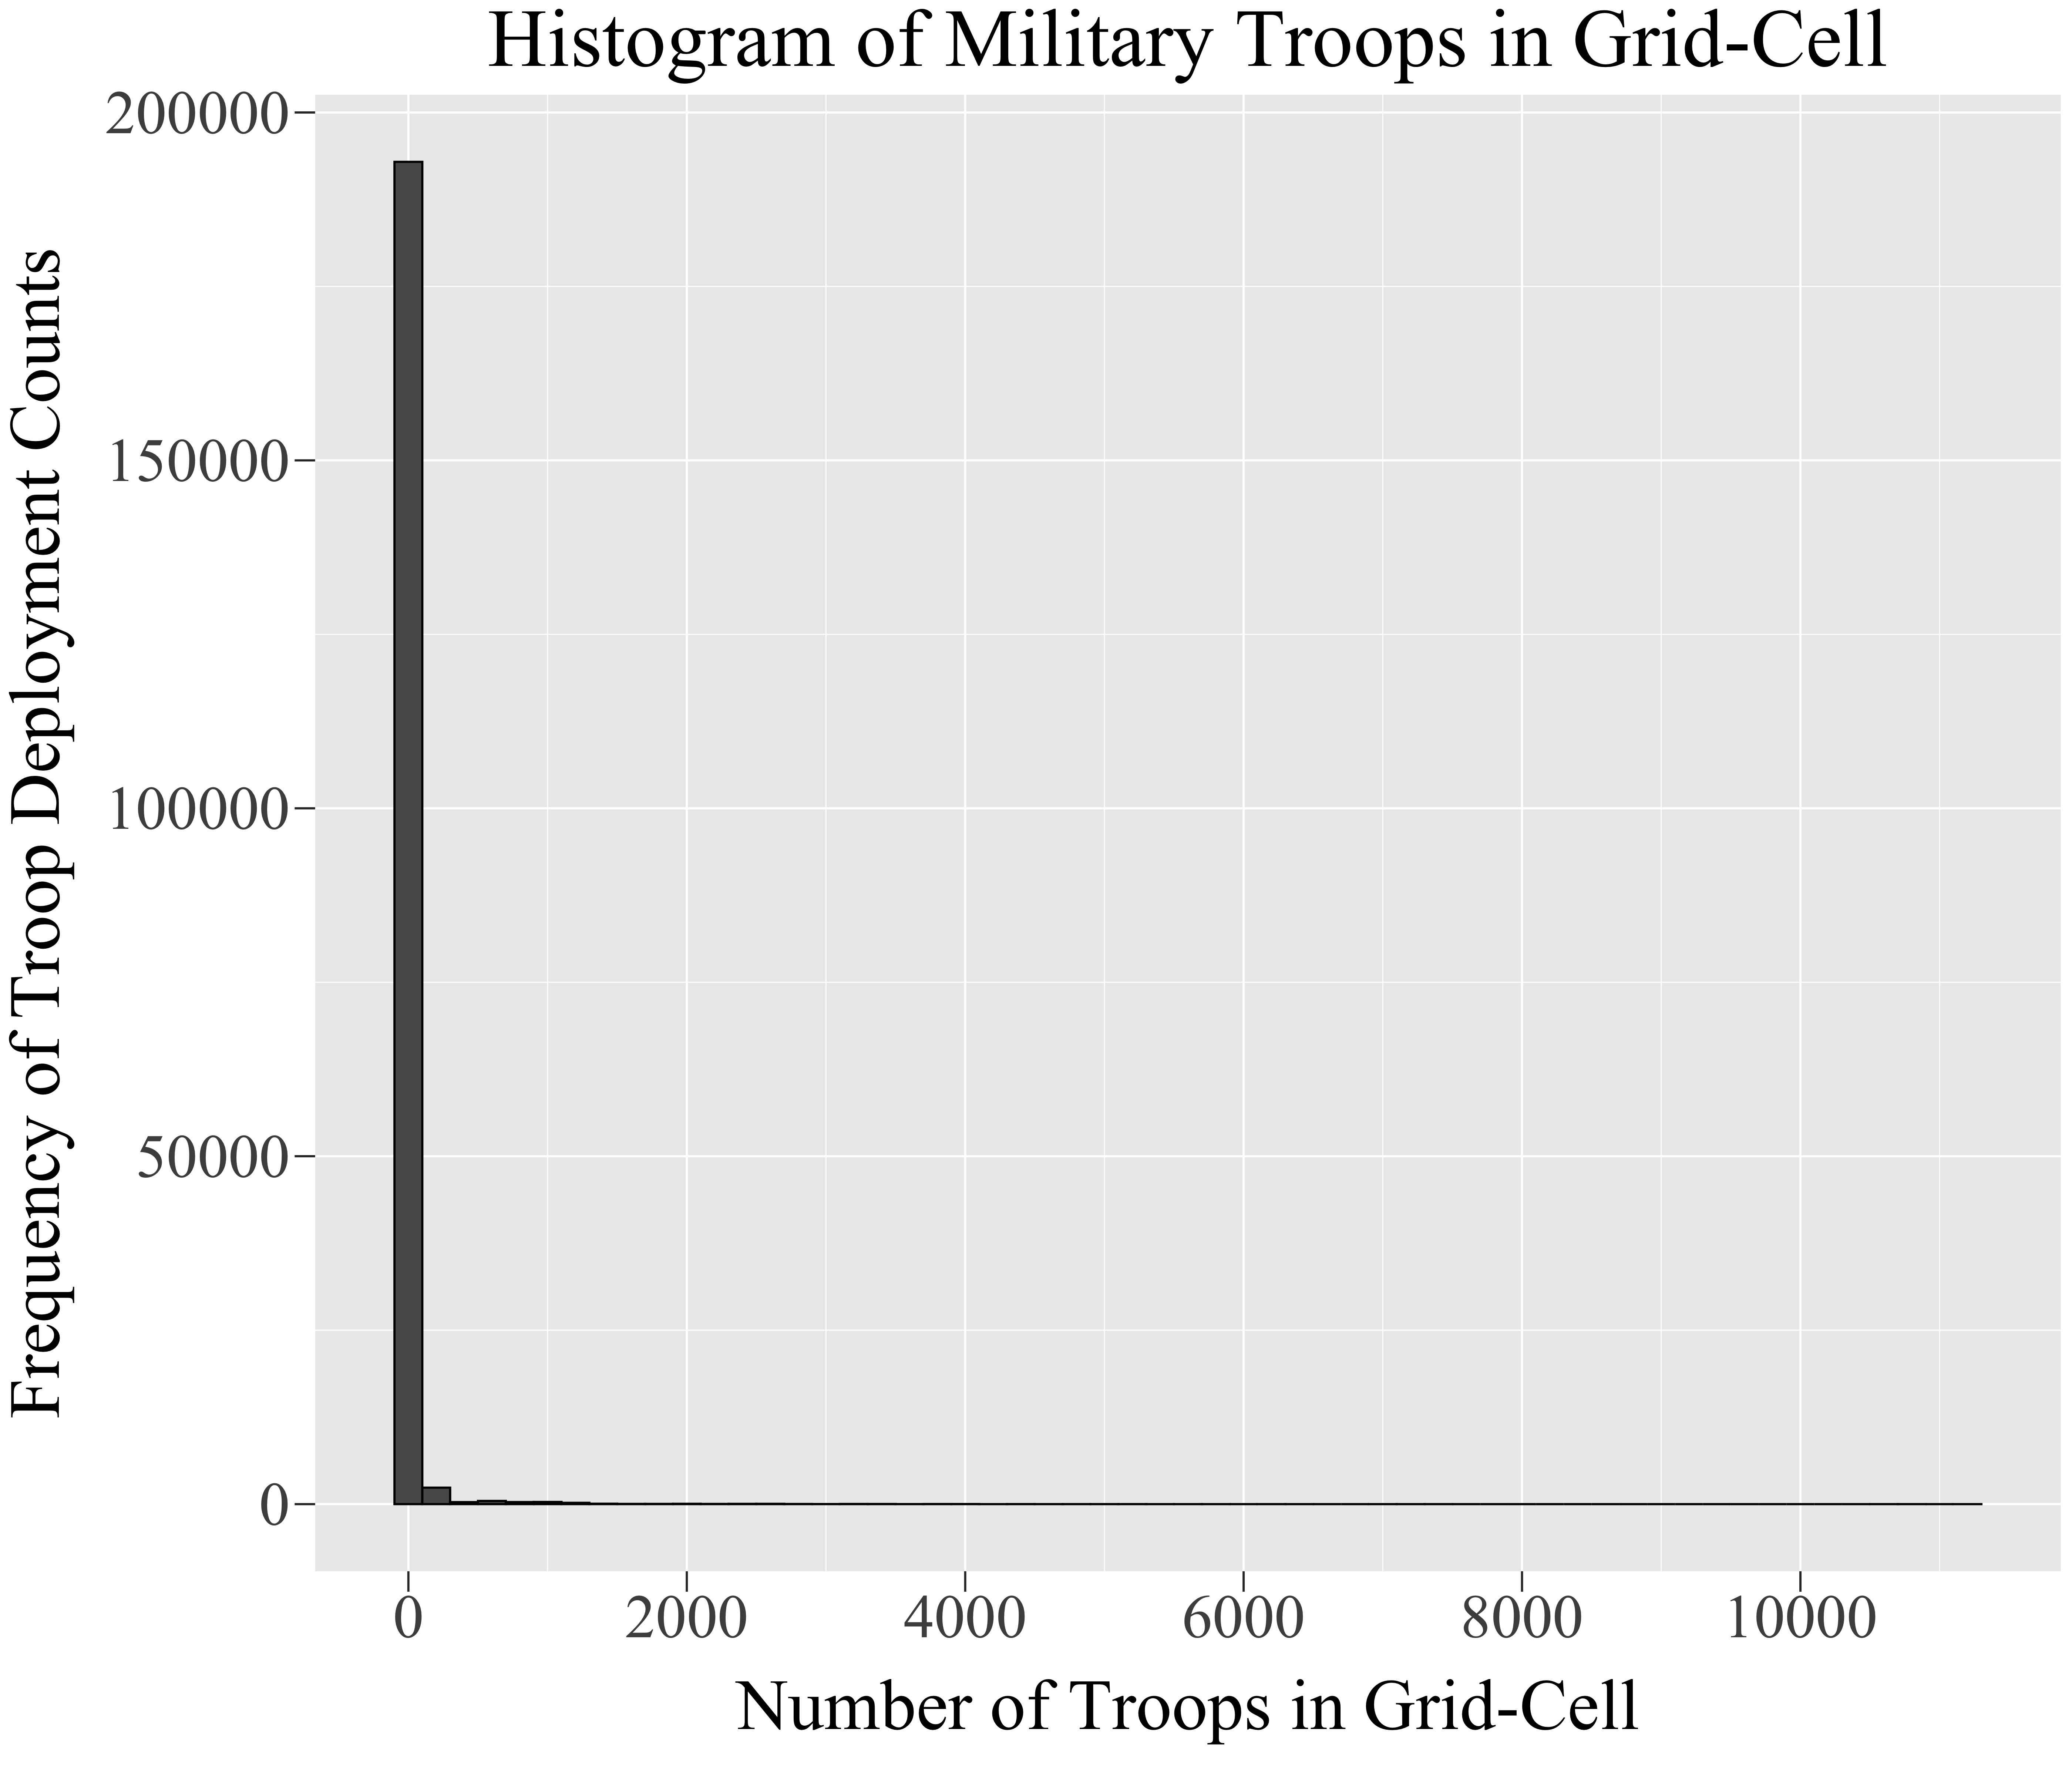
\includegraphics[width=\linewidth]{gg_Hist_DV.jpg}
\caption{Histogram of Troops}
\end{subfigure}
\hfill
\begin{subfigure}[h]{0.5\linewidth}
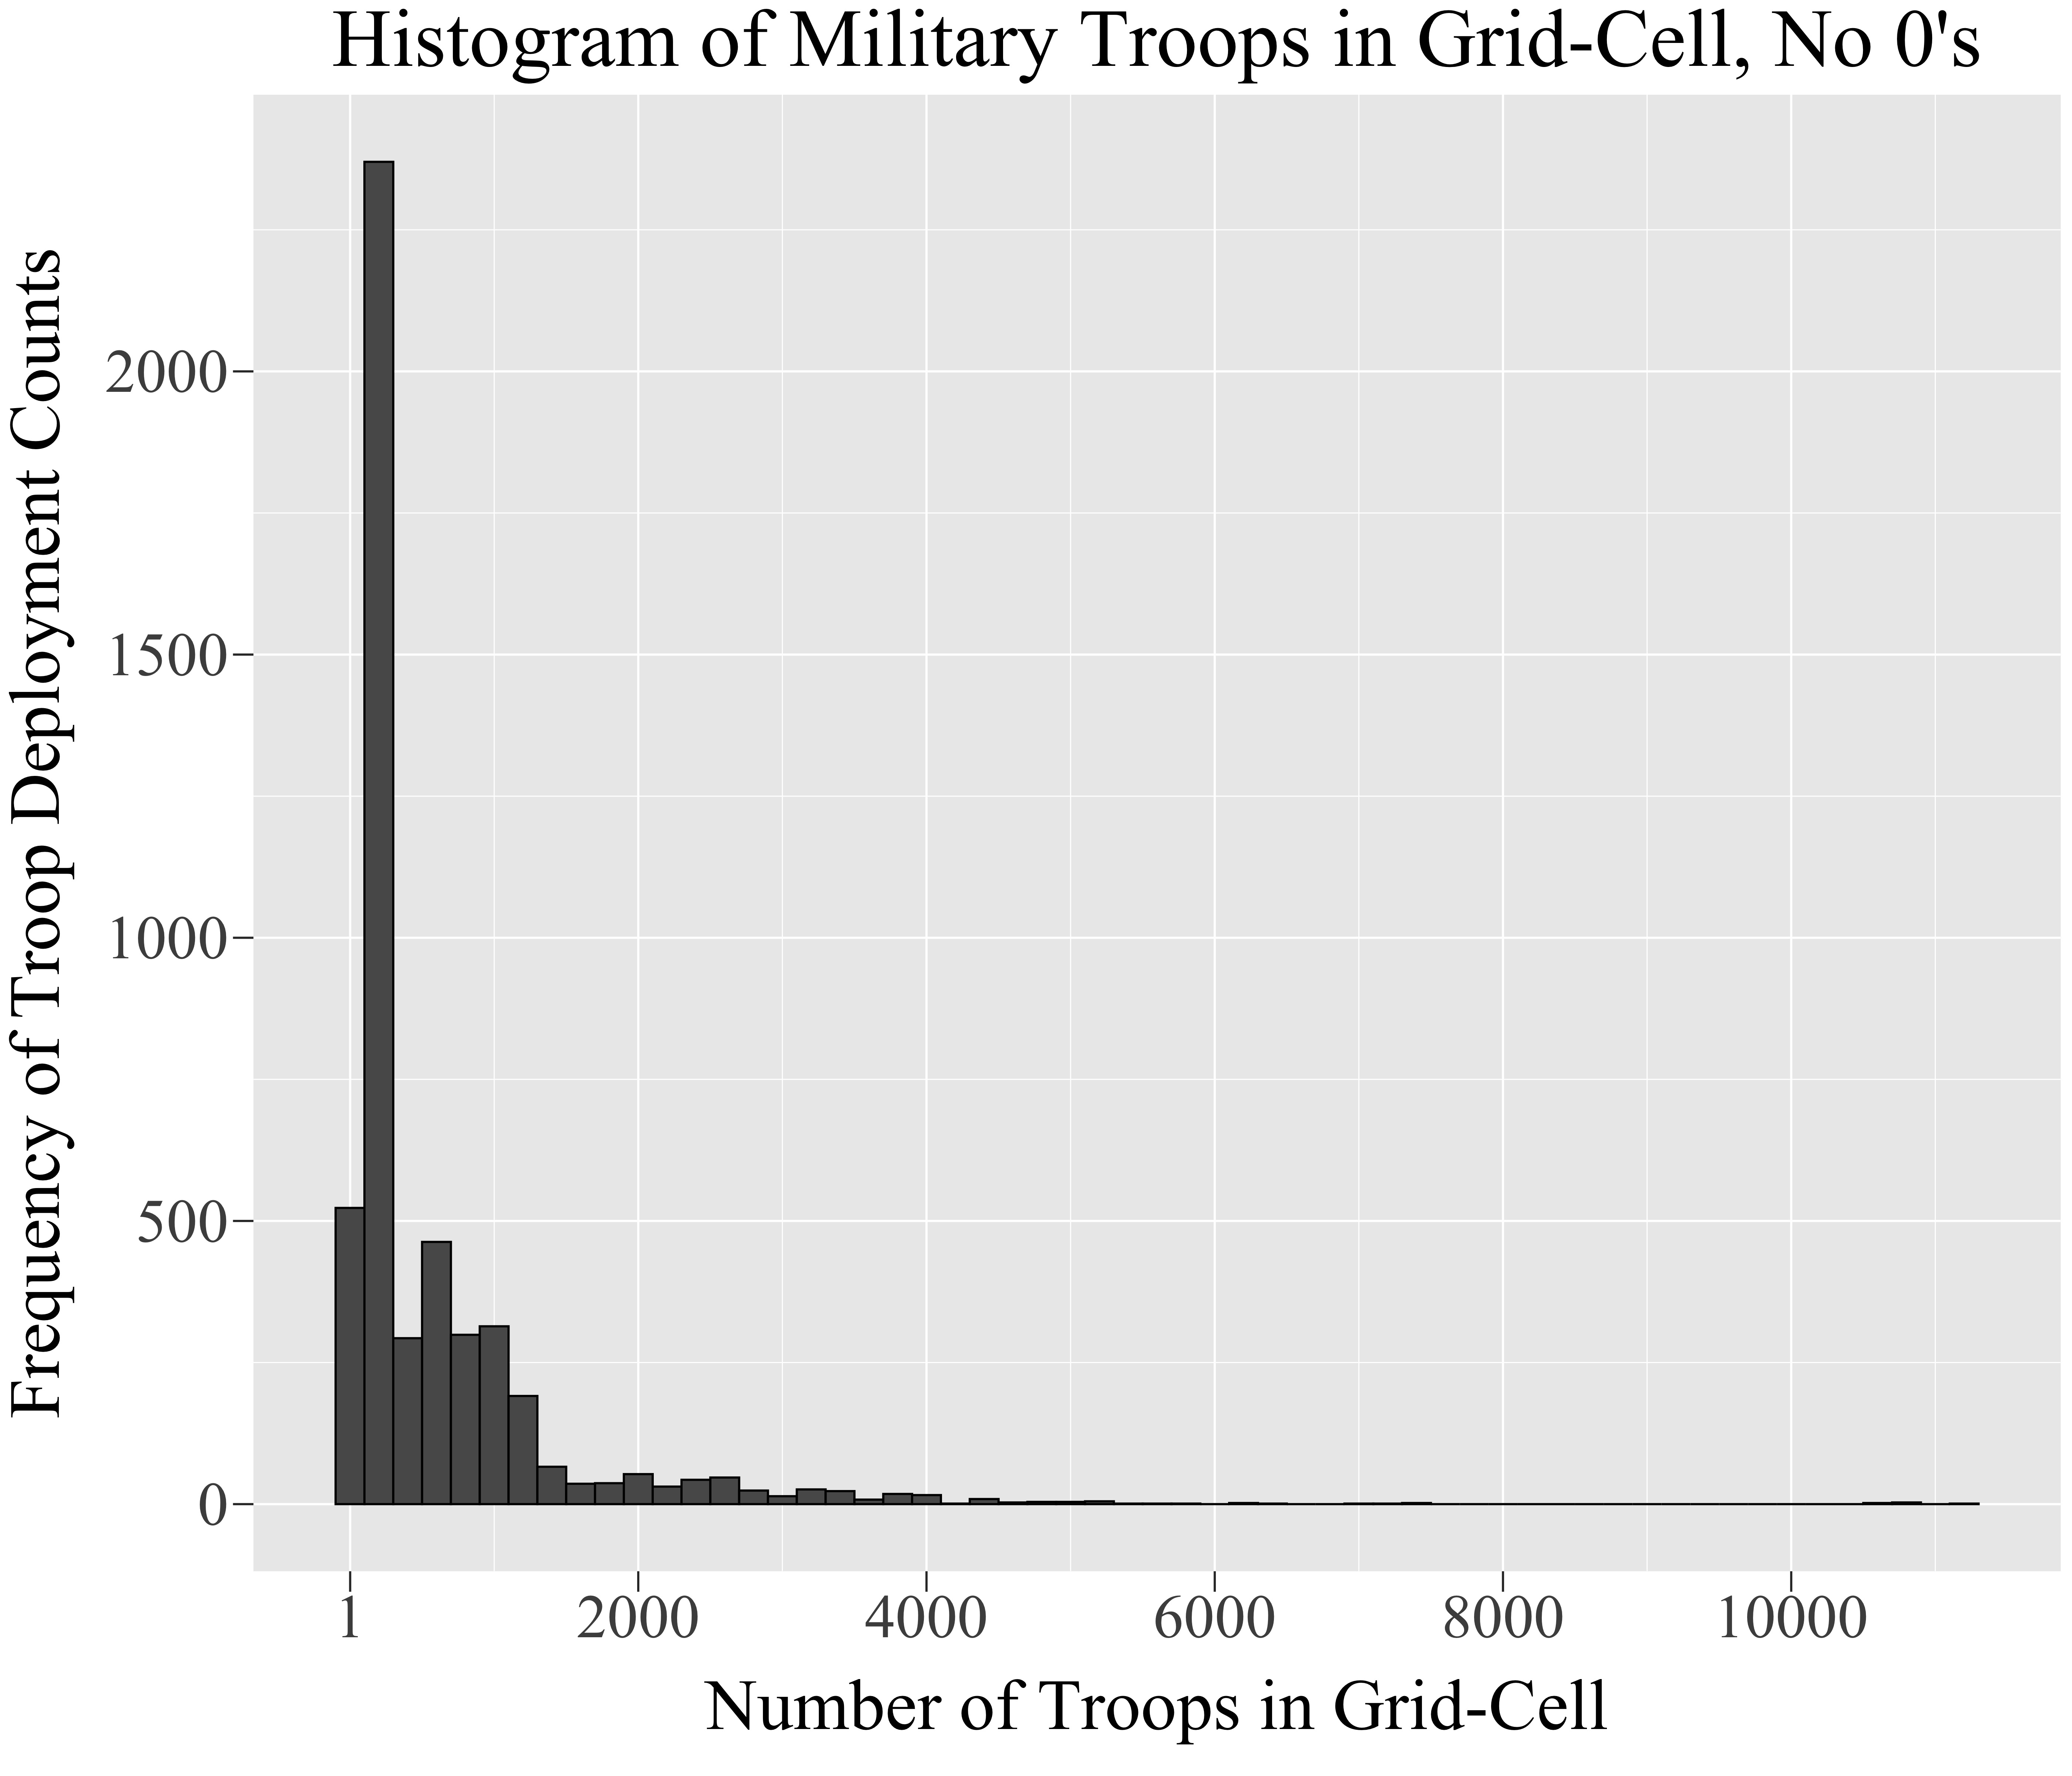
\includegraphics[width=\linewidth]{gg_Hist_DV_No_0.jpg}
\caption{Histogram of Troops, No 0's}
\end{subfigure}%
\caption{\small Histograms of the troop contributions.}
% 5 words
\label{fig:Figure 1}
\end{figure}
\end{comment}

\clearpage

%%% Regression Table %%%
\begin{comment}
\begin{centering}
\begin{table}[htbp]\centering
\footnotesize
\def\sym#1{\ifmmode^{#1}\else\(^{#1}\)\fi}
\caption{The Effect of Risk Ratio on Contributions \label{Table 2}}
\begin{tabular}{l*{5}{c}}
\hline\hline
                    &\multicolumn{1}{c}{Model 1} &\multicolumn{1}{c}{Model 2} &\multicolumn{1}{c}{Model 3} &\multicolumn{1}{c}{Model 4} &\multicolumn{1}{c}{Model 5}        \\
\hline
Risk Ratio$_{t-1}$          &      -1.601\sym{**}&      -2.103\sym{**}&      -1.875\sym{**}&      -1.250\sym{**}&      -1.179\sym{**}\\
                    &     (0.498)        &     (0.459)        &     (0.477)        &     (0.444)        &     (0.457)        \\
[0.5em]
Battle Deaths$_{t-1}$ (Hundreds)&       0.012        &       0.072        &       2.359\sym{**}&       0.087        &       0.929        \\
                    &     (0.085)        &     (0.099)        &     (0.636)        &     (0.104)        &     (0.668)        \\
Risk Ratio$_{t-1}$ X Battle Deaths$_{t-1}$&                    &                    &      -3.086\sym{**}&                    &      -1.150        \\
                    &                    &                    &     (0.858)        &                    &     (0.940)        \\
[0.5em]
Troop Shortfall$_{t-1}$ (Hundreds)&                    &                    &                    &       0.015\sym{**}&       0.015\sym{**}\\
                    &                    &                    &                    &     (0.002)        &     (0.002)        \\
[0.5em]
Number of Contributors$_{t-1}$ (Tens)&                    &      -0.069\sym{\dagger} &      -0.073\sym{\dagger} &      -0.099\sym{**}&      -0.100\sym{**}\\
                    &                    &     (0.036)        &     (0.038)        &     (0.038)        &     (0.038)        \\
[0.5em]
Re-hatted$_{t-1}$           &                    &      -0.045        &      -0.043        &      -0.131        &      -0.130        \\
                    &                    &     (0.156)        &     (0.155)        &     (0.169)        &     (0.169)        \\
[0.5em]
Previous UN Mission$_{t-1}$ &                    &       0.555\sym{**}&       0.539\sym{**}&       0.486\sym{**}&       0.479\sym{**}\\
                    &                    &     (0.132)        &     (0.133)        &     (0.156)        &     (0.156)        \\
[0.5em]
Contributor GDP per Capita$_{t-1}$ (Ten Thousands)&                    &      -0.114\sym{*} &      -0.114\sym{*} &      -0.110\sym{*} &      -0.110\sym{*} \\
                    &                    &     (0.053)        &     (0.052)        &     (0.050)        &     (0.050)        \\
[0.5em]
Contributor Democracy$_{t-1}$&                    &       2.324\sym{**}&       2.290\sym{**}&       2.315\sym{**}&       2.304\sym{**}\\
                    &                    &     (0.501)        &     (0.500)        &     (0.512)        &     (0.513)        \\
[0.5em]
Total Contributed Troops$_{t-1}$ (Hundreds)&                    &       0.027\sym{**}&       0.026\sym{**}&       0.020\sym{**}&       0.020\sym{**}\\
                    &                    &     (0.009)        &     (0.009)        &     (0.007)        &     (0.007)        \\
[0.5em]
Proportion of Contributor Troops$_{t-1}$&                    &       1.109\sym{\dagger} &       1.108\sym{\dagger} &       1.462\sym{\dagger} &       1.459\sym{\dagger} \\
                    &                    &     (0.576)        &     (0.575)        &     (0.773)        &     (0.771)        \\
[0.5em]
Same Continent$_{t-1}$      &                    &      -0.004        &       0.005        &      -0.160        &      -0.155        \\
                    &                    &     (0.170)        &     (0.166)        &     (0.176)        &     (0.174)        \\
[0.5em]
Trade$_{t-1}$ (Billions)    &                    &       0.168\sym{*} &       0.162\sym{*} &       0.314\sym{**}&       0.310\sym{**}\\
                    &                    &     (0.080)        &     (0.076)        &     (0.118)        &     (0.117)        \\
[0.5em]
Joint IOs$_{t-1}$           &                    &       0.020\sym{**}&       0.019\sym{**}&       0.020\sym{**}&       0.020\sym{**}\\
                    &                    &     (0.007)        &     (0.007)        &     (0.007)        &     (0.007)        \\
[0.5em]
Troops$_{t-1}$              &       0.632\sym{**}&       0.519\sym{**}&       0.519\sym{**}&       0.551\sym{**}&       0.550\sym{**}\\
                    &     (0.093)        &     (0.083)        &     (0.083)        &     (0.092)        &     (0.092)        \\
[0.5em]
Constant            &       3.529\sym{**}&       1.833\sym{**}&       1.707\sym{**}&       0.987        &       0.953        \\
                    &     (0.430)        &     (0.604)        &     (0.602)        &     (0.627)        &     (0.623)        \\
\hline
lnalpha             &       2.056\sym{**}&       1.884\sym{**}&       1.882\sym{**}&       1.753\sym{**}&       1.752\sym{**}\\
                    &     (0.099)        &     (0.090)        &     (0.090)        &     (0.089)        &     (0.089)        \\
\hline
Observations        &       78659        &       72553        &       72553        &       61665        &       61665        \\
\hline\hline
\multicolumn{6}{l}{\footnotesize State clustered standard errors in parentheses}\\
\multicolumn{6}{l}{\footnotesize Dependent variable is troop counts. 15 potential contributor random sample.}\\
\multicolumn{6}{l}{\footnotesize \sym{\dagger} \(p<0.10\), \sym{*} \(p<0.05\), \sym{**} \(p<0.01\). Two-tailed test.}\\
\end{tabular}
\end{table}

\end{centering}
\end{comment}

\clearpage

%%% H1 margins plots %%%

\begin{comment}
\begin{figure}[t!]
\begin{centering}
\includegraphics[width=110mm]{gg_M2.jpg}
\caption{Predicted troop contribution counts with 95\% confidence intervals based on Model 2.}
\label{fig:Figure 2}
\end{centering}{}
\end{figure}
\end{comment}

\clearpage

%%% H2 marginal effects plot %%%

\begin{comment}
\begin{figure}[t!]
\begin{centering}
\includegraphics[width=110mm]{gg_M3.jpg}
\caption{\small Evaluating the conditional effects of risk ratio and battle deaths with 95\% confidence intervals from Model 3. For reference, the mean count of battle deaths per contributor-mission-month is about 15 deaths. The average contribution is about 178 troops.}
% 40 words
\label{fig:Figure 3}
\end{centering}
\end{figure}
\end{comment}

\clearpage 

%%% Task Marginal effects %%%

\begin{comment}
\begin{figure}[t!]
\begin{centering}
\includegraphics[width = 180mm, height = 100mm]{coef.jpg}
\caption{Risky Task Marginal Effects}
% 6 words
\label{fig:Figure 4}
\end{centering}
\end{figure}
\end{comment}

\clearpage % Page break to seperate the work from the bibliography. 
%\singlespacing

\bibliographystyle{chicago} % My citation style is APSR

\bibliography{/Users/treywood/Dropbox/Projects/Active_Projects/Mandate_Contribute/Paper/PKO.bib} % This locates my bibliographic information



\end{document}